\documentclass[12pt]{article}

\usepackage{appendix}
\usepackage[french]{babel}
\usepackage[utf8]{inputenc}
\usepackage[normalem]{ulem}
\usepackage[T1]{fontenc}
\usepackage{listings}
\usepackage{graphicx}
\usepackage{xcolor}
\usepackage[a4paper, total={6.5in, 10.5in}]{geometry}
\usepackage{float}
\usepackage[colorlinks = true, allcolors = blue]{hyperref}

\renewcommand{\appendixpagename}{Annexes}
\renewcommand{\appendixtocname}{Annexes}
\graphicspath{ {./images/} }

\definecolor{mGreen}{rgb}{0,0.6,0}
\definecolor{mGray}{rgb}{0.5,0.5,0.5}
\definecolor{mPurple}{rgb}{0.58,0,0.82}
\definecolor{backgroundColour}{rgb}{0.95,0.95,0.92}

\lstdefinestyle{PythonStyle}{
    backgroundcolor = \color{backgroundColour},   
    commentstyle = \color{mGreen},
    keywordstyle = \color{magenta},
    numberstyle = \tiny\color{mGray},
    stringstyle = \color{mPurple},
    basicstyle = \footnotesize,
    breakatwhitespace = false,         
    breaklines = true,                 
    captionpos = b,                    
    keepspaces = true,                 
    numbers = left,                    
    numbersep = 5pt,                  
    showspaces = false,                
    showstringspaces = false,
    showtabs = false,                  
    tabsize = 2,
    language = Python
}

\lstdefinestyle{save}{
    backgroundcolor = \color{backgroundColour},
    numbers = left
}

\begin{document}

\title{
    \rule{\linewidth}{0.3mm} \\[0.4cm]
    { \huge \bfseries Projet de Programmation 2025 - Rapport Final \\ \large Hex - Python \\ Master 1 Informatique \\[0.4cm] }
    \rule{\linewidth}{0.3mm} \\[0.4cm]}
\author{KUSTERS Timon \\ HERR Mariano \\ ROCHETEAU Yohann \\ GUITARD Paul \\ HUBINCU Morgan}
\date{}
\begin{figure}
    \centering
    
\includegraphics[width=0.5\linewidth]{logo.png}
    \label{fig:logo}
\end{figure}

\maketitle
\newpage
\tableofcontents

\newpage
\section{Règles du jeu}

Le jeu de Hex est un jeu de plateau se basant sur de la stratégie, sans notion de hasard ou de chance. Une partie se joue sur un plateau en forme de losange régulier (carré), remplis de cases hexagonales. La partie se joue à deux joueurs, ayant pour l'un des pions blancs et pour l'autre des pions noirs. Chaque joueur se voit attribuer deux bordures parallèles du plateau. Le but du jeu est de les connecter via une ligne de pions hexagonaux contigus de sa propre couleur, en plaçant un pion chacun à son tour sur n'importe quelle case, à la seule condition que cette dernière soit libre. Selon le théorème de Nash (\cite{VVA2002}), le match nul n'existe pas, un joueur parvient toujours à joindre ses deux bordures de plateau avant que celui-ci ne soit complètement rempli.

\begin{figure}[H]
    \centering
    
\includegraphics[width=0.75\linewidth]{hex.png}
    \caption{Image montrant une partie de Hex sur notre interface graphique gagnée par le joueur ayant les pions noirs.}
    \label{fig:hex}
\end{figure}

\section{Existant du projet}

Faisant uniquement appel à la logique, le jeu de Hex est un bon problème pour tester et développer des algorithmes de recherche et leurs heuristiques en IA. De nombreux papiers présentent des méthodes, des outils et des approches manipulant ce jeu. Des compétitions entre plusieurs joueurs artificiels ont eu lieu, comparant les efficacités des algorithmes des compétiteurs. C'est le cas des outils MoHex \cite{AHH10} et Yopt \cite{DBLP:journals/ria/CazenaveS09} qui implémentent la recherche arborescente Monte-Carlo. Quelques heuristiques y sont discutées. Un article en compile quelques-unes \cite{RJ02} et \cite{RJ00} dont two distances (bfs) et potential threats que nous utilisons (cf. heuristiques \ref{heuristiques}). Ces articles ont servi à implémenter la recherche arborescente Monte Carlo et des heuristiques pour notre joueur artificiel.

\bigskip
En ce qui concerne le jeu de base, le plateau est souvent implémenté à l'aide de tableau en deux dimensions \cite{playhex} ou par un graphe \cite{JAhex} ou par une structure permettant l'union rapide pondérée \cite{Abdo}. Le plateau du jeu de Hex peut aussi, comme de nombreux autres jeux comme le Go ou les échecs, être représenté par des bitboards. Des méthodes communes à ces jeux ont été créées et explicitées par Browne \cite{browne14} dont une qui permet la détection de connexions qui marque la fin de partie dans le jeu de Hex. L'algorithme présenté, le bitwise-parallel reduction \cite{browne12}, utilise une Y-réduction qui est une structure qui peut être obtenue à partir de bitboards et permet des opérations vectorielles entre les colonnes du plateau. Nous avons repris l'algorithme de Browne \cite{browne12} et avons noté la pertinence d'utiliser l'union rapide pondérée dans la détection de connexion (cf. critiques \ref{crit-connec}).

\newpage
\section{Principaux algorithmes et structures utilisés}

\subsection{Plateau et Bitboards}

\subsubsection{Structure}

\begin{lstlisting}[style = PythonStyle]
class Board:
    def __init__(self, dim: int):
    	self.__dim = dim
    	self.__size = dim * dim
    	self.__wbits = Bitboard(self.__size)
    	self.__bbits = Bitboard(self.__size)
\end{lstlisting}

\bigskip
Le plateau de jeu est représenté par deux bitboards, un pour chaque joueur. Ces bitboards représentent deux mots binaires qui stockent pour chacun la position des pièces d’un des deux joueurs. Un bit représente une case, la taille des bitboards (en bits) est donc la dimension du plateau au carré. Cela permet un usage faible de la mémoire. De plus, les bitboards, implémentés en héritant du module bitarray, permettent les opérations sur bits telles que |, \&, $<<$, etc. Des lectures et écritures efficaces et des calculs vectoriels peuvent donc être utilisés. Par exemple, la méthode check\_legal\_move(position) de cette classe, qui renvoie un booléen selon si le coup représenté par sa position est légal ou illégal, utilise l’opération sur bit  $\neg(self.\_\_wbits | self.\_\_bbits)$ pour obtenir, en un seul calcul, le bitboard des cases vides où le joueur peut jouer. Par souci de lisibilité, lors des accès aux bitboards, les mots binaires sont en little endian afin que bits[0] représente la première case du plateau. Pour les détails des méthodes, voir section implémentation.

\subsubsection{Détection de connexion} \label{algo-bpr}

L’algorithme le plus important, appelé à chaque fois qu’un coup est joué, et qui justifie donc l’usage des bitboards pour le rendre plus efficace, est celui de la détection de connexion qui marque la fin de la partie.
Pour cela, on utilise une Y-réduction \cite{browne12}. Dans la structure utilisée par cet algorithme, le plateau est représenté par un bitboard pour chaque colonne, et les cases du plateau sont représentées par une paire de bits : “00” pour une case vide, “01” pour une case blanche, “10” pour une case noire, “11” pour les cases inutilisées. Cette méthode fait perdre un peu d’espace mémoire (on passe de deux bitboards à dim + 1 bitboards, dim étant la dimension du plateau du jeu, par exemple 13 dans un jeu de hex de taille 13x13) mais on garde les opérations sur bit. La détection se fera comme ceci : 

\bigskip
\textbf{(a)} On convertit les bitboards en une Y-réduction. Pour cela, on parcourt les bits des deux bitboards en ajoutant, si le bit d’un des deux bitboards est à 1, 2 bits (correspondant au codage ci-dessus) à la position $2^{2 \times i}$. Les bitboards sont parcourus par ligne, donc on construit 2 bits de chaque colonne toutes les dim tours de boucles. On ajoute une autre colonne en plus des dim colonnes ainsi que 2 bits en plus pour chaque colonne qui vont représenter le template du jeu (les bords). Dans la figure \ref{fig:y-red-struct} et dans notre implémentation, les cases en noir valent “10”, en blanc “01”, en gris clair “11” et les cases en gris foncé sont remplies selon le plateau. Cette conversion sera faite à chaque fois que l’on veut détecter une connexion. La conversion est faite en O(dim²) ou en O(n) si n représente la taille des bitboards. Un rapport de performance est disponible (section performances \ref{perf}) pour montrer le coup de cette opération en pratique.

\bigskip
\begin{figure}[H]
    \centering
    
\includegraphics[width=0.8\linewidth]{/Y-reduction-structure.png}
    \caption{Figure montrant la structure obtenue après la conversion (à droite) et la structure après dim pas de calcul (à gauche). Figure altérée de \cite{browne12}. En plus du codage explicité précédemment, en gris très foncé sont représentées les cases qui n'ont plus d'information et dont la valeur qu'elles contiennent n'est pas importante.}
    \label{fig:y-red-struct}
\end{figure}

\bigskip
\textbf{(b)} On utilise ensuite cette structure en la passant à l’algorithme BPR suivant :
\begin{lstlisting}[style = PythonStyle]
def bitwise_parallel_reduction(bits: list[Bitboard], dim: int) -> GameOverState:
    cols = 2 * dim - 1
    pas = 0
    while pas < cols - 1:
        col = 0
        while col < (min(dim + 1, cols - pas) - 1):
            a = bits[col]
            b = (a << 2)  # SE neighbors
            c = bits[col+1]  # E neighbors
            bits[col] = (a & (b | c)) | (b & c)
            col += 1
        pas += 1
    if bits[0].get_bit(1) == 1:
        return GameOverState.BLACK_WON
    if bits[0].get_bit(0) == 1:
        return GameOverState.WHITE_WON
    return GameOverState.NO_WINNER
\end{lstlisting}

\bigskip
Le principe est de réduire les triplets d’hexagones en un seul, qui contient la majorité des couleurs. Ici, on effectue cette opération à chaque pas sur toute une colonne en même temps, en utilisant l’opération (a \& (b | c)) | (b \& c) qui renvoie la couleur majoritaire (cf. figure \ref{fig:y-red}) du triplet. ‘a’ représente la colonne traitée,’ b‘ la même colonne, mais décalée vers le bas par rapport à la figure pour représenter les voisins au Sud-Est, et ‘c‘ est la colonne directement à droite par rapport à la figure représentant les voisins à l’Est.

\bigskip
\begin{figure}[H]
    \centering
    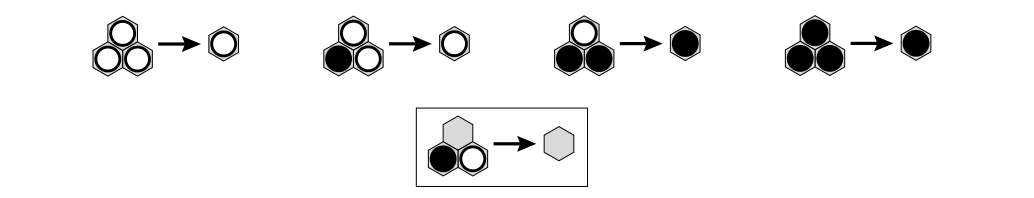
\includegraphics[width=0.8\linewidth]{y_reduction.png}
    \caption{Les différentes sorties que produit l'opération sur bit (a \& (b | c)) | (b \& c). Figure de \cite{browne12}.}
    \label{fig:y-red}
\end{figure}

\bigskip
cols - 1 représente le nombre de pas nécessaire pour réduire l’entièreté du tableau. Ce nombre est égal à $2 \times dim - 1$ qui est la distance de Manhattan entre la première case et la dernière case du plateau (la case en gris foncé en haut à droite de la figure). Ce nombre de pas est nécessaire afin que l’information se trouvant dans la dernière case soit communiquée jusqu’à la première case.

\bigskip
Depuis le point de vue de cette dernière case, à chaque pas, l’information se répand une case vers la gauche puis au prochain pas une case vers le bas. C’est pour cela que la diagonale en haut à droite de la structure peut être considérée comme “traitée”, car elle n’a plus d’information. C’est aussi pour cela que, après que la moitié des pas aient été effectués et qu’il ne reste qu’un “triangle rectangle”, il ne reste qu’une seule case possédant une information sur l’avant-dernière colonne. À partir de ce moment, il devient donc possible d’ignorer cette colonne, d’où la condition $col < (min(dim + 1, cols - pas) - 1)$ (-1, car la dernière colonne ne sert qu’à être lue).
À la fin, le résultat se retrouve dans les 2 bits de la première case. On renvoie donc, selon le codage défini au-dessus, un état de fin de partie correspondant au gagnant.

\bigskip
Lors d’un jeu avec un ou deux joueurs artificiels, les limites de cette solution apparaissent (cf. performances \ref{perf}). Des solutions existent (cf. critiques \ref{crit-connec}), ce problème de performance a malheureusement été découvert trop tard.

\subsection{Historiques des coups joués/annulés}

La classe History représente l'historique des coups joués et annulés, en ayant pour attributs deux listes (done\_moves et undone\_moves). Outre les détails techniques, les deux listes sont manipulées de manière similaire à une double pile : jouer un coup ajoute ce dernier dans la pile des coups joués (via un dictionnaire permettant de récupérer le joueur, la position et les temps de ce dernier), et il est possible de transvaser ce coup d’une pile à l’autre via un undo ou un redo. Aussi, jouer un coup réinitialise (vide) la liste des coups annulés.

\subsection{IA : Algorithmes d’exploration}

\subsubsection{Minimax \& Alpha-Beta}

Minimax et Alpha-Beta sont deux algorithmes d’exploration d'arbres utilisant une heuristique pour simuler tous les états, et remonter la meilleure valeur (le meilleur coup). Alpha-Beta étant une optimisation de Minimax, on s’intéresse donc à ce dernier dans un premier temps. Minimax part du principe que le joueur pour lequel on calcule, que l’on appellera “ami”, cherche à jouer le meilleur coup possible, donc le coup avec le plus haut score possible. En opposition à ami, nous avons le joueur ennemi, qui lui cherche à récupérer le plus bas score possible. Ce principe est possible, car le jeu de Hex est un jeu à somme nulle : ce que gagne un joueur, son adversaire le perd. Calculer la plus grosse perte de l'ennemi revient donc à calculer le plus gros gain de ami. On définit alors une profondeur maximale qui représente le nombre de tours que l’on va regarder. Cela revient à regarder ce qu’il se passera dans le futur pour savoir quel coup nous avantage le plus. Enfin, on remonte les scores calculés depuis les états feuilles de l'arbre, sachant que lorsque c’est à ami de jouer, on récupère le maximum parmi les valeurs possibles.

\bigskip
\begin{figure}[H]
    \centering
    \includegraphics[width=0.8\linewidth]{Minmax.png}
    \caption{Schéma montrant le déroulement de Minimax sur un arbre fictif (\href{https://commons.wikimedia.org/wiki/File:Min_Max_Sample_1.png}{source}). La couche B joue le rôle de l'ennemi et sélectionne le minimum des valeurs possibles, et la couche A sélectionne le maximum des minimums.}
    \label{fig:MinMax}
\end{figure}

\bigskip
Alpha-Beta vient rajouter deux variables à l’algorithme Minimax : alpha et beta. Alpha correspond à la meilleure valeur que Ami (joueur MAX) peut garantir à un moment donné, et beta à la meilleure valeur que Ennemi (joueur MIN) peut garantir. Lors du tour d’Ami, on met à jour alpha si l’on trouve une valeur plus grande que le alpha courant, et pendant celui d’Ennemi, on met à jour beta si l’on trouve une valeur plus petite que le beta courant. Ces variables permettent un élagage de l’arbre des coups possibles, ce qui améliore fortement les performances, car on évite d’explorer des nœuds inutiles. Cet élagage a lieu lorsque alpha >= beta, car cela signifie qu’une autre branche est déjà meilleure pour le joueur parent, et que la branche courante ne sera jamais choisie. Par exemple, si Ami peut déjà garantir un score de 6 (alpha = 6) et qu’Ennemi peut forcer un score de 5 (beta = 5), Ami ignorera cette branche. Notre implémentation d'Alpha-Beta a été réalisée en s'inspirant de l’optimisation Negamax \cite{alpha} qui, pour comparer les nœuds, inverse le signe des fils. 

\bigskip
\begin{figure}[H]
    \centering
    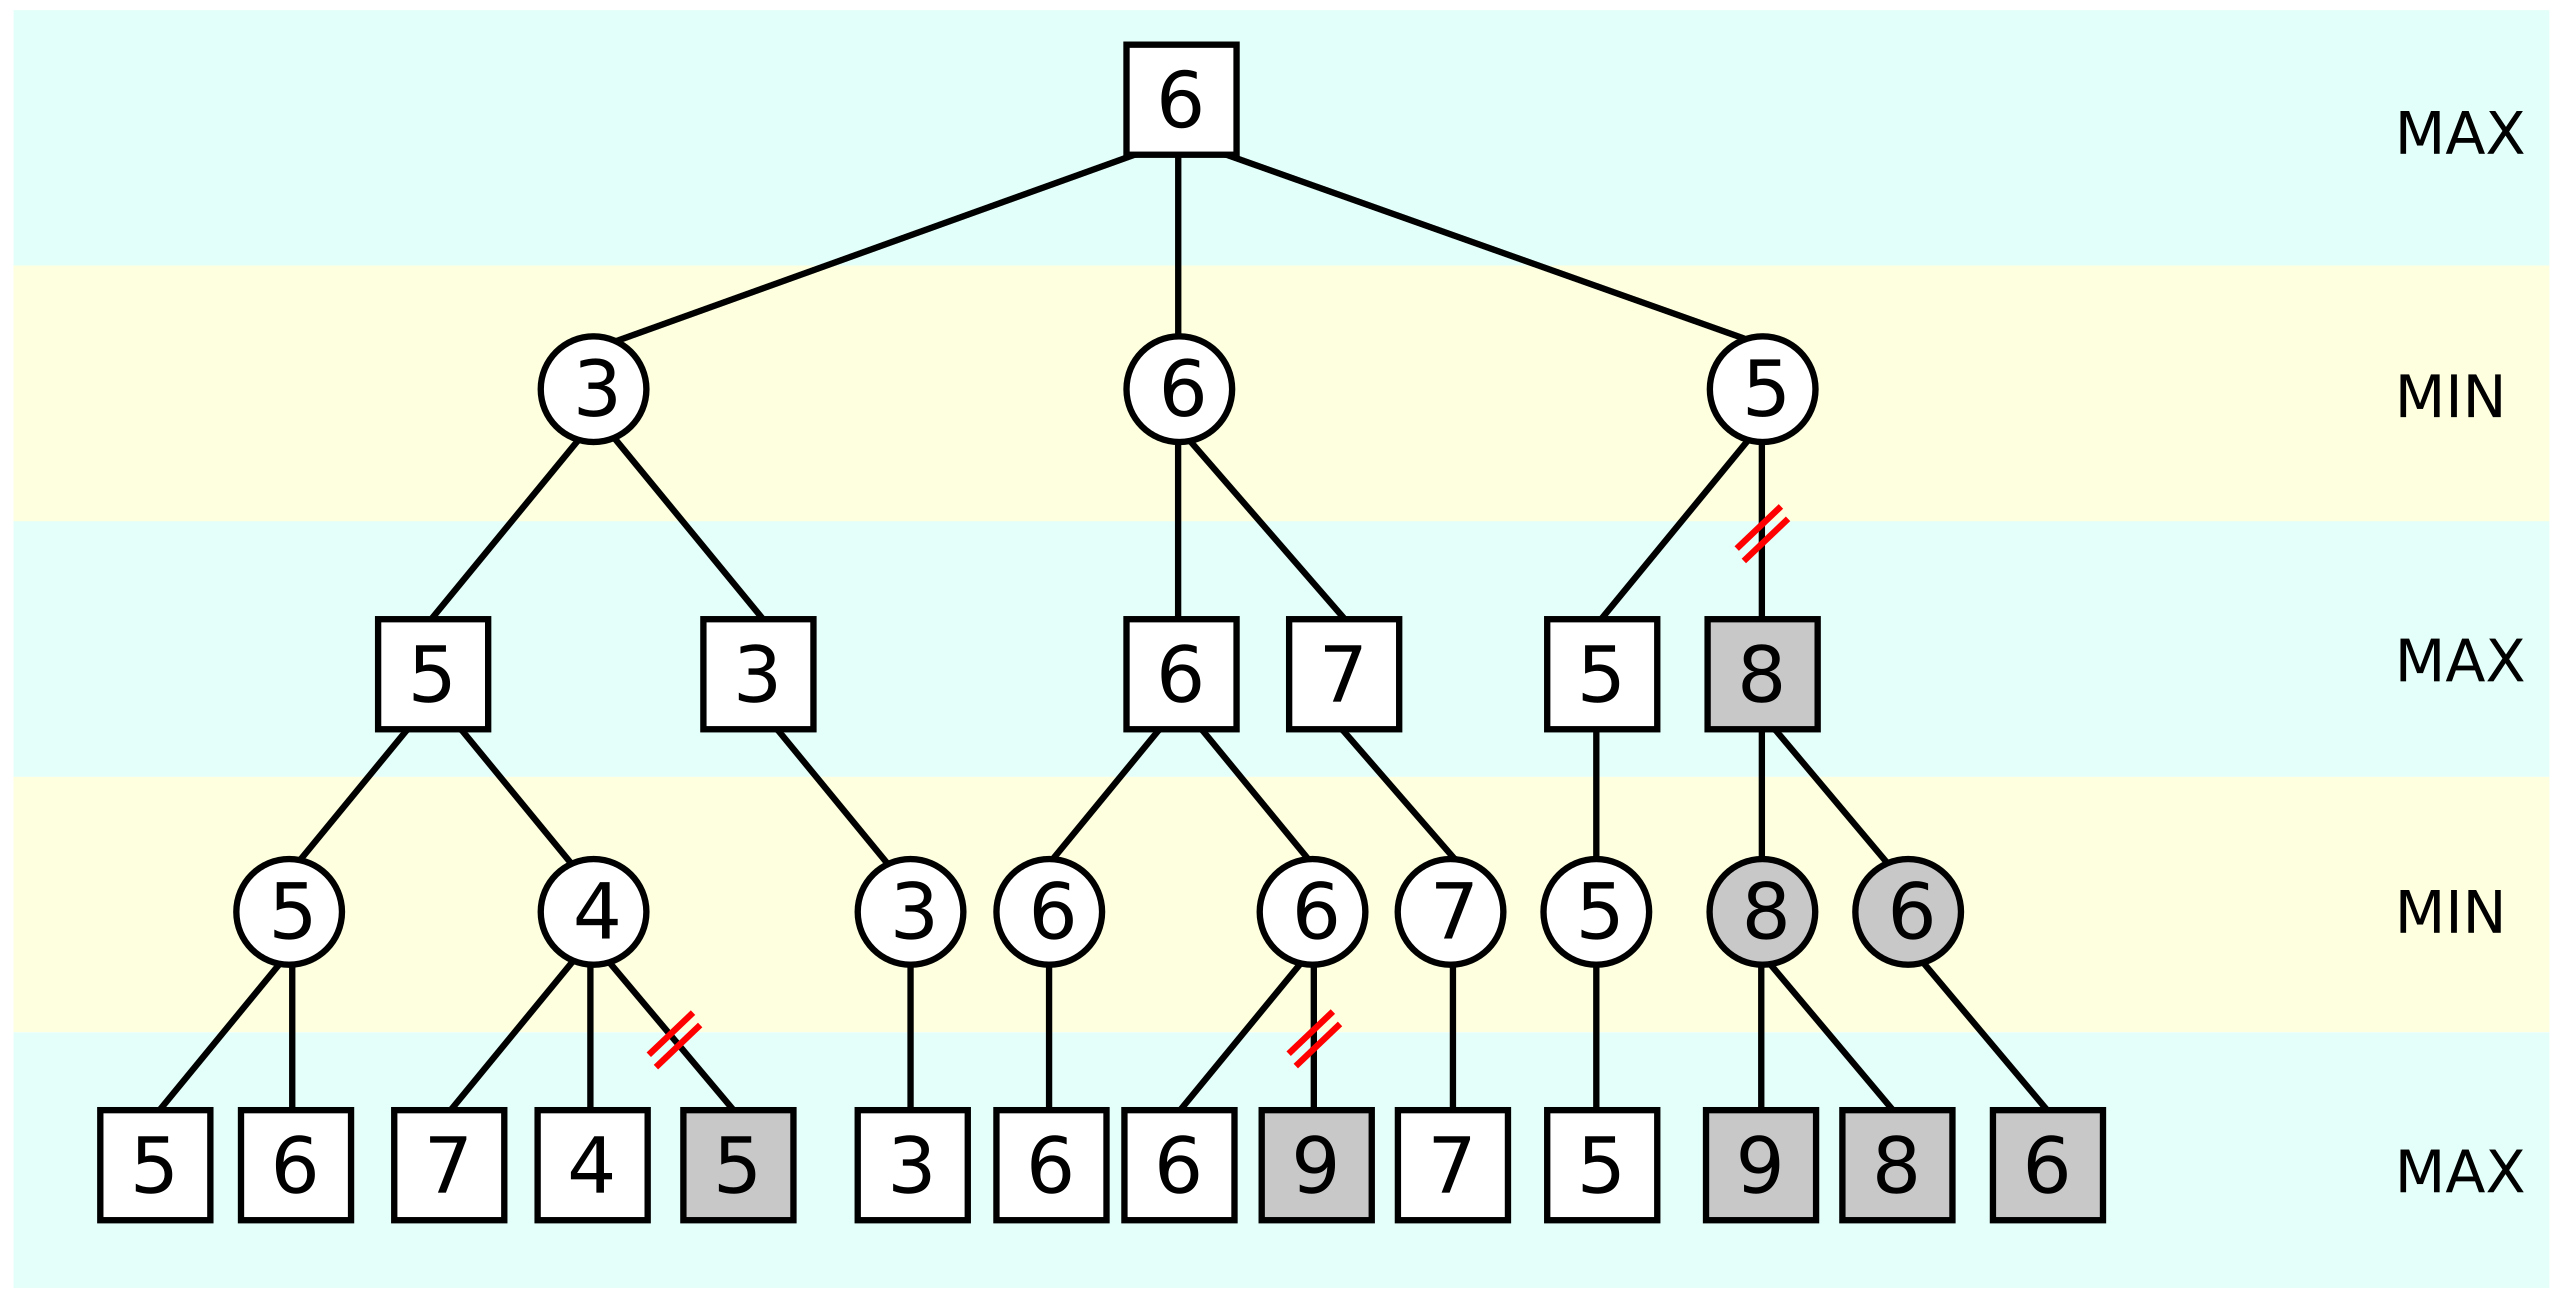
\includegraphics[width=0.8\linewidth]{AlphaBeta.png}
    \caption{Schéma montrant le déroulement d'Alpha-Beta sur un arbre fictif (\href{https://commons.wikimedia.org/wiki/File:Poda_alfa-beta.svg}{source}, illustration par \href{https://commons.wikimedia.org/wiki/User:Willtron}{Willtron}. \href{https://creativecommons.org/licenses/by-sa/3.0/deed.en}{Licence}). On voit bien que considérer la partie la plus à droite de l’arbre est inutile, car MAX garantira un score de 6 alors que MIN garantira un score d’au maximum 5.}
    \label{fig:AlphaBeta}
\end{figure}

\subsubsection{Monte Carlo Tree Search}

Monte Carlo Tree Search est un algorithme de recherche utilisé dans les jeux pour déterminer les meilleurs coups à jouer. Il repose sur des simulations aléatoires de parties pour estimer la valeur d’un coup, sans avoir besoin de parcourir tout l’arbre des possibilités. L’idée est de favoriser les actions qui semblent prometteuses tout en continuant à en explorer d'autres de temps en temps. Pour cela, l’algorithme répète quatre étapes :

\bigskip
\begin{itemize}
    \item Sélection : à partir de la racine, on descend dans l’arbre en suivant les coups les plus prometteurs. Pour déterminer quel coup est le plus prometteur, on se base sur la formule UCT \cite{DBLP:journals/ria/CazenaveS09}.
    \item Expansion : lorsqu’un nœud qui n'est pas encore totalement exploré est atteint, on ajoute un nouveau coup.
    \item Simulation : on joue une partie aléatoire complète à partir de ce coup.
    \item Rétro propagation : le résultat de la simulation est remonté jusqu’à la racine pour mettre à jour les statistiques des nœuds visités.
\end{itemize}

\bigskip
\begin{figure}[H]
    \centering
    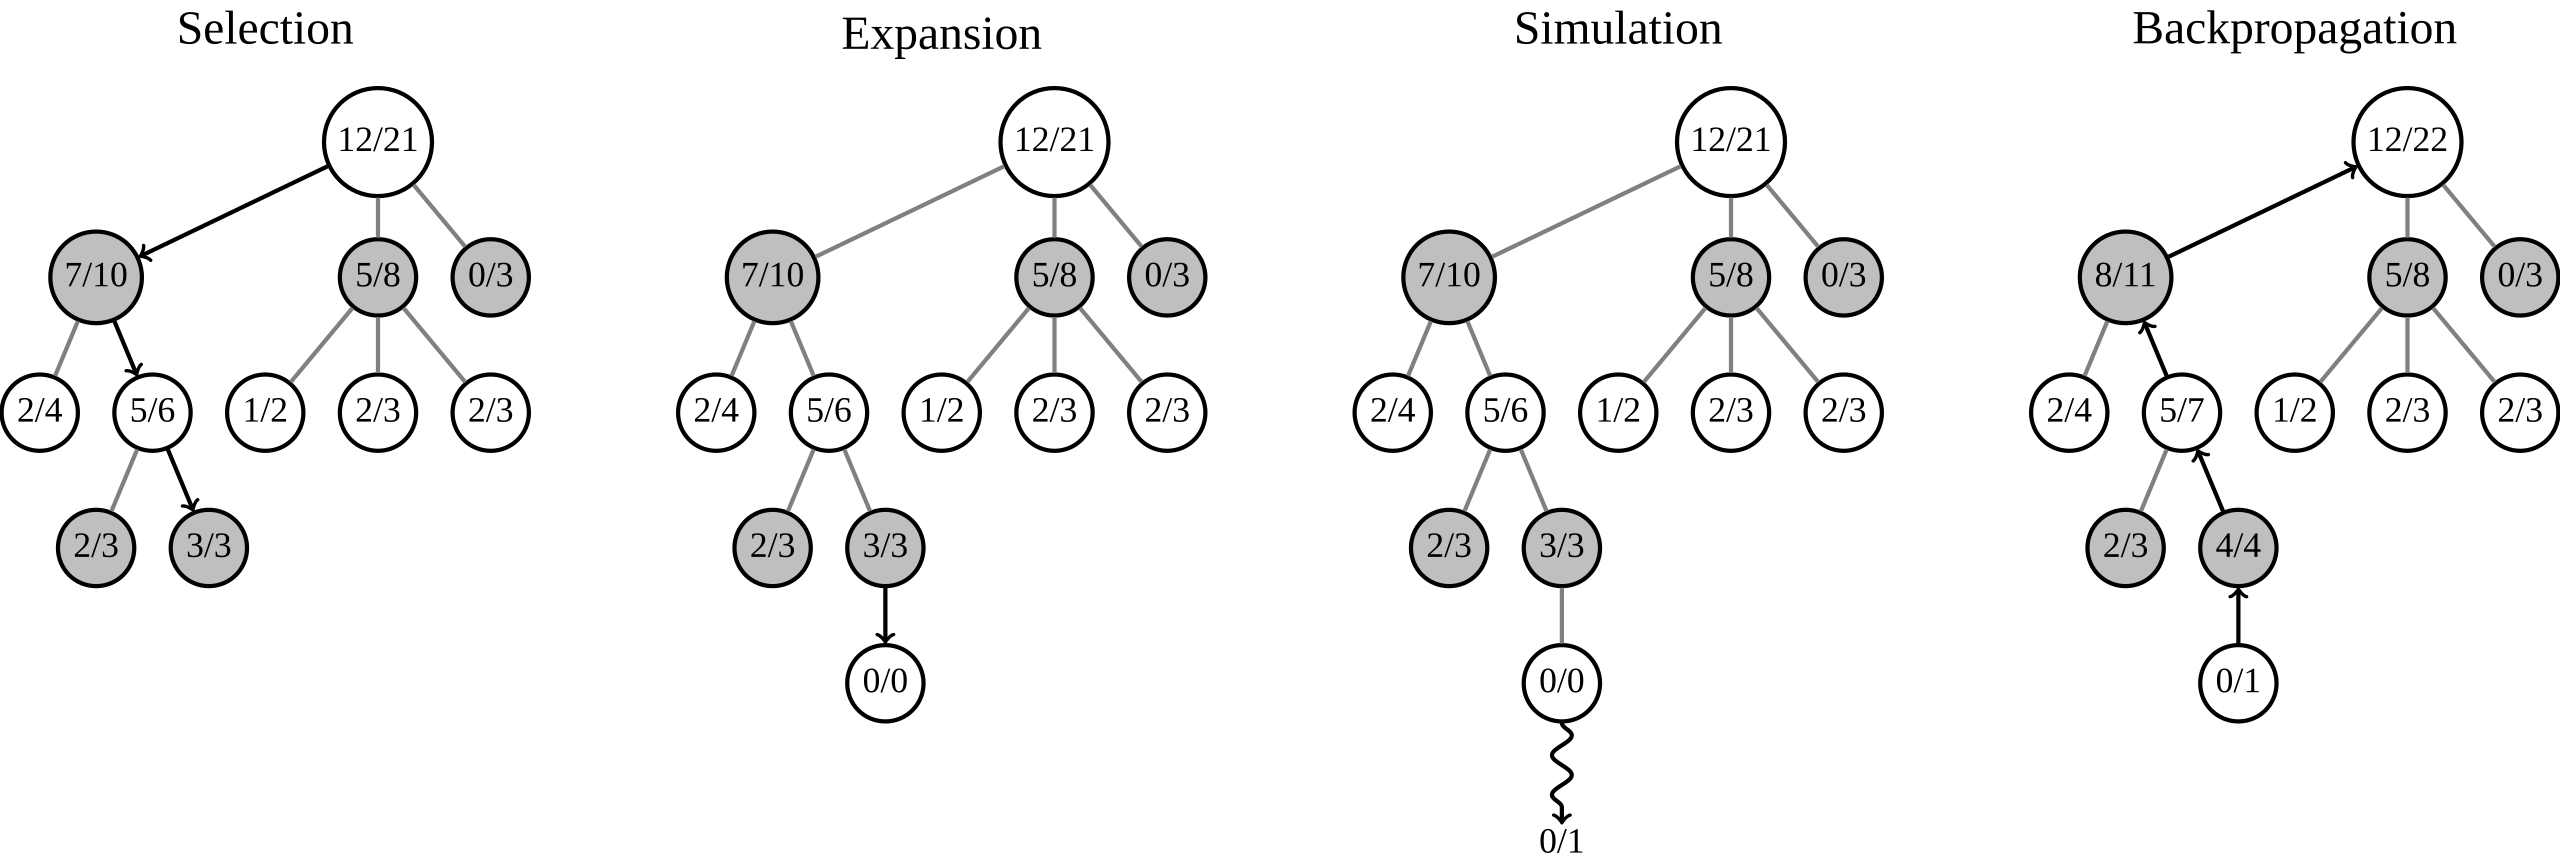
\includegraphics[width=1\linewidth]{MCTS.png}
    \caption{Schéma montrant le déroulement de MCTS sur un arbre fictif (\href{https://commons.wikimedia.org/wiki/File:MCTS_(French).svg}{source})}.
    \label{fig:MCTS}
\end{figure}

\subsection{IA : Heuristiques} \label{heuristiques}

\subsubsection{Dijkstra} \label{algo-dijkstra}

Pour cette heuristique, on se base sur l’algorithme de Dijkstra \cite{dijk} pour calculer la distance d’un point par rapport à un objectif. L'objectif est représenté par la dernière ligne ou dernière colonne selon le joueur qui évalue le plateau. On estime le coût minimum du chemin pour gagner. Pour se faire, on crée deux tableaux de la même taille que notre plateau de jeu. Un tableau (update) indique quelle case n’a pas été mise à jour, pour laquelle on devra donc calculer son coût. L’autre tableau contient le coût de chaque chemin. Au final, on obtient le coût minimum de l’adversaire et du joueur pour gagner. On renvoie donc le couple coût adversaire - coût joueur. Plus la valeur de retour est haute, plus le plateau est favorable pour le joueur.

\subsubsection{Potential Threats}

Pour cette heuristique, on s'inspire de l'algorithme “Potentials” de la thèse de Jack van Rijswijck \cite{RJ00}. Le principe est que, pour relier deux côtés du plateau, on souhaite chercher la tuile qui est la plus proche possible d’être connectée aux deux extrémités cibles. On va donc appeler "potentiel" la valeur représentant à quel point il est possible pour un joueur de joindre ses deux extrémités. Là où on diffère de la source est pour la seconde métrique que l’on va implémenter. Dans l’article, on parle de mobilité de l’attaque, qui définit à quel point plusieurs tuiles peuvent réaliser le plus grand potentiel.Par soucis de simplicité et de temps, on va ajouter une métrique que l’on appellera "menace", qui compte le nombre de tuiles que l’adversaire peut relier pour bloquer le joueur. L’avantage de cette formule est qu'il est simple de donner une directive à l’heuristique, en ajoutant des poids pour chaque métrique.

\subsubsection{Path oriented heuristic} \label{path_oritented}

L’objectif pour cette heuristique est d'assurer la victoire en calculant plusieurs métriques qui semblent intéressantes pour gagner. Pour ceci, on va privilégier les coups au centre du plateau, le prolongement de chemin existant, les tuiles dans les zones critiques (tel que le centre et les extrémités) et à quel point l’adversaire est proche de gagner. On transforme ces valeurs en un score qui agit tel une pénalité, que l’on va soustraire au score final. De plus, on rajoute un poids à chacun des scores qui va dépendre de l’avancement de la partie. Pour savoir l’avancement de la partie, on compare la taille des coups légaux par rapport à la taille du plateau, et l’on ajoute une pénalité aux coups isolés pour privilégier la continuation de notre chemin. Par exemple, en fin de partie, on préfère se concentrer sur le prolongement de son propre chemin et bloquer l’adversaire plutôt que de prendre en compte les zones sont moins importantes.

\bigskip
On divise le calcul du score en 5 valeurs:

\begin{itemize}
    \item Score de pont: on récompense les endroits où un "pont" (lien) peut être créé : deux pièces avec une case vide entre (inspiré de \cite{AHH10}).
    \item Zones critiques: on définit des zones critiques, les extrémités et le centre, et on pénalise l’adversaire s'il possède ces zones, ou on récompense le joueur s'il en possède.
    \item Prolongation du chemin: selon le joueur, on favorise les coups qui prolongent les chemins dans la bonne direction.
    \item Menace du joueur ennemi: On pénalise le plateau si l’adversaire est plus proche de finir que le joueur.
    \item Pièce isolée: On pénalise les plateaux avec des pièces isolées, car elles ont moins de chance de contribuer à la victoire.
\end{itemize}

\bigskip
On additionne les scores et on soustrait les pénalités, ce qui nous donne le score du plateau final. Le désavantage majeur de cette heuristique est le nombre de paramètres. En effet, chaque score possède une valeur qui s’incrémente lorsque le plateau "performe" dans un critère. De plus, on a 3 poids par score. On a donc plus d’une vingtaine d’hyper-paramètres. La performance de cette heuristique est grandement affectée par ces derniers, ce qui peut être chronophage à perfectionner.

\subsubsection{BFS}

Cette heuristique est plus simple et naïve que les autres. Elle se base sur un parcours en largeur qui calcule la plus courte distance jusqu’à l’arrivée. On normalise le calcul en fonction de la taille du plateau, ce qui nous donne un score entre 0 et 1. Pour avoir la propriété que "plus le score est élevé plus il est profitable au joueur", on soustrait la distance minimale trouvée, normalisée à 1. Selon le joueur, on retourne le score de l'ennemi auquel on soustrait celui de score ami pour avoir une valeur qui sera plus élevée en fonction de si le plateau profite plus à ami qu’à ennemi.

\newpage
\section{Architecture du projet}

\subsection{Architecture générale}

Pour notre projet, nous n'avons pas suivi de modèle standard (MVC, DDD, etc.), mais nous avons regroupés les module par catégories de répertoires:
\begin{itemize}
    \item hex.tools : regroupe les fichiers de "fonctionnalités" du jeu et non liés à l'affichage ou à l'IA (timers, fichiers, historiques, etc.).
    \item hex.userinterfaces : regroupe les fichiers liés à l'affichage du jeu (CLI et GUI).
    \item hex.ai : regroupe tous les fichiers liés à l'IA.
\end{itemize}

\bigskip
\begin{figure}[H]
    \centering
    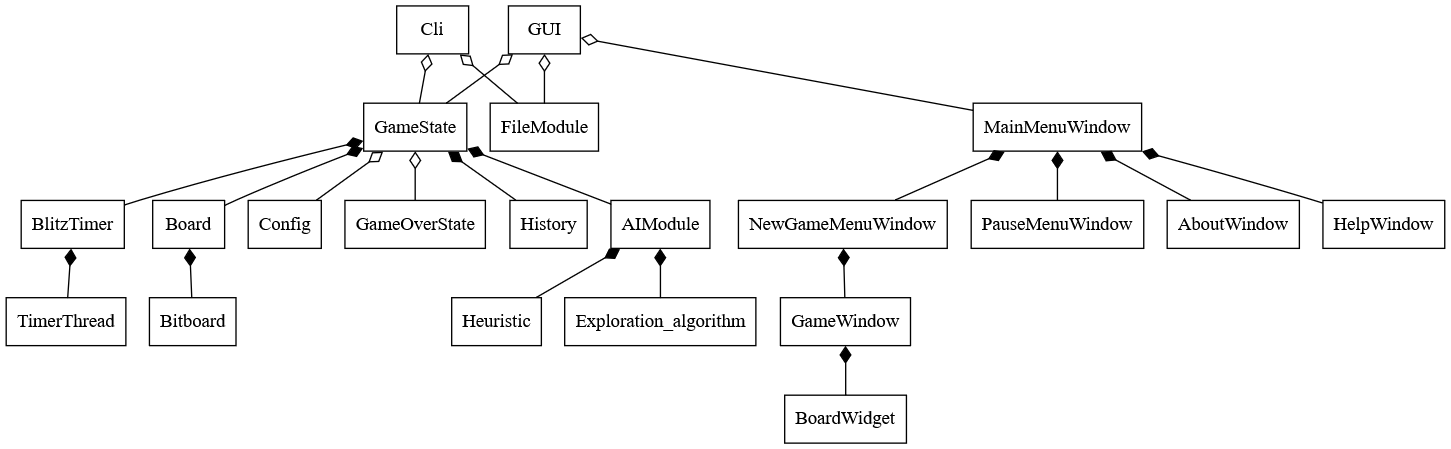
\includegraphics[width=1\linewidth]{images/UML_hex.png}
    \caption{Diagramme UML de l'ensemble du projet.}
    \label{fig:UML_hex}
\end{figure}

\subsection{hex.tools}

Le répertoire hex.tools regroupe l'ensemble des fichiers servant d'utilitaires. Ces derniers sont liés via la classe GameState, qui peut faire office de modèle et de contrôleur. Le GUI ou le CLI possèdent tous deux une instance de cette classe, à laquelle ils font appel lorsque les données du jeu doivent être mises à jour avant de rafraîchir l'affichage. GameState contient donc nombre de méthodes pour récupérer des données ou faire des actions. Par exemple, lorsque l'on cherche à jouer un coup (play\_move()), il regarde si ce dernier est valide avant de le placer dans le plateau (module Board). Entre autres, il met aussi à jour les historiques (module History) avant de renvoyer une valeur au GUI ou au CLI servant à mettre à jour l'affichage de façon adéquate.

\bigskip
Pour le module Board, comme les algorithmes de détection de connexions et de recherche de chemin gagnant sont dans des modules à part, il peuvent facilement être interchangés avec d'autres si désiré.

\bigskip
\begin{figure}[H]
    \centering
    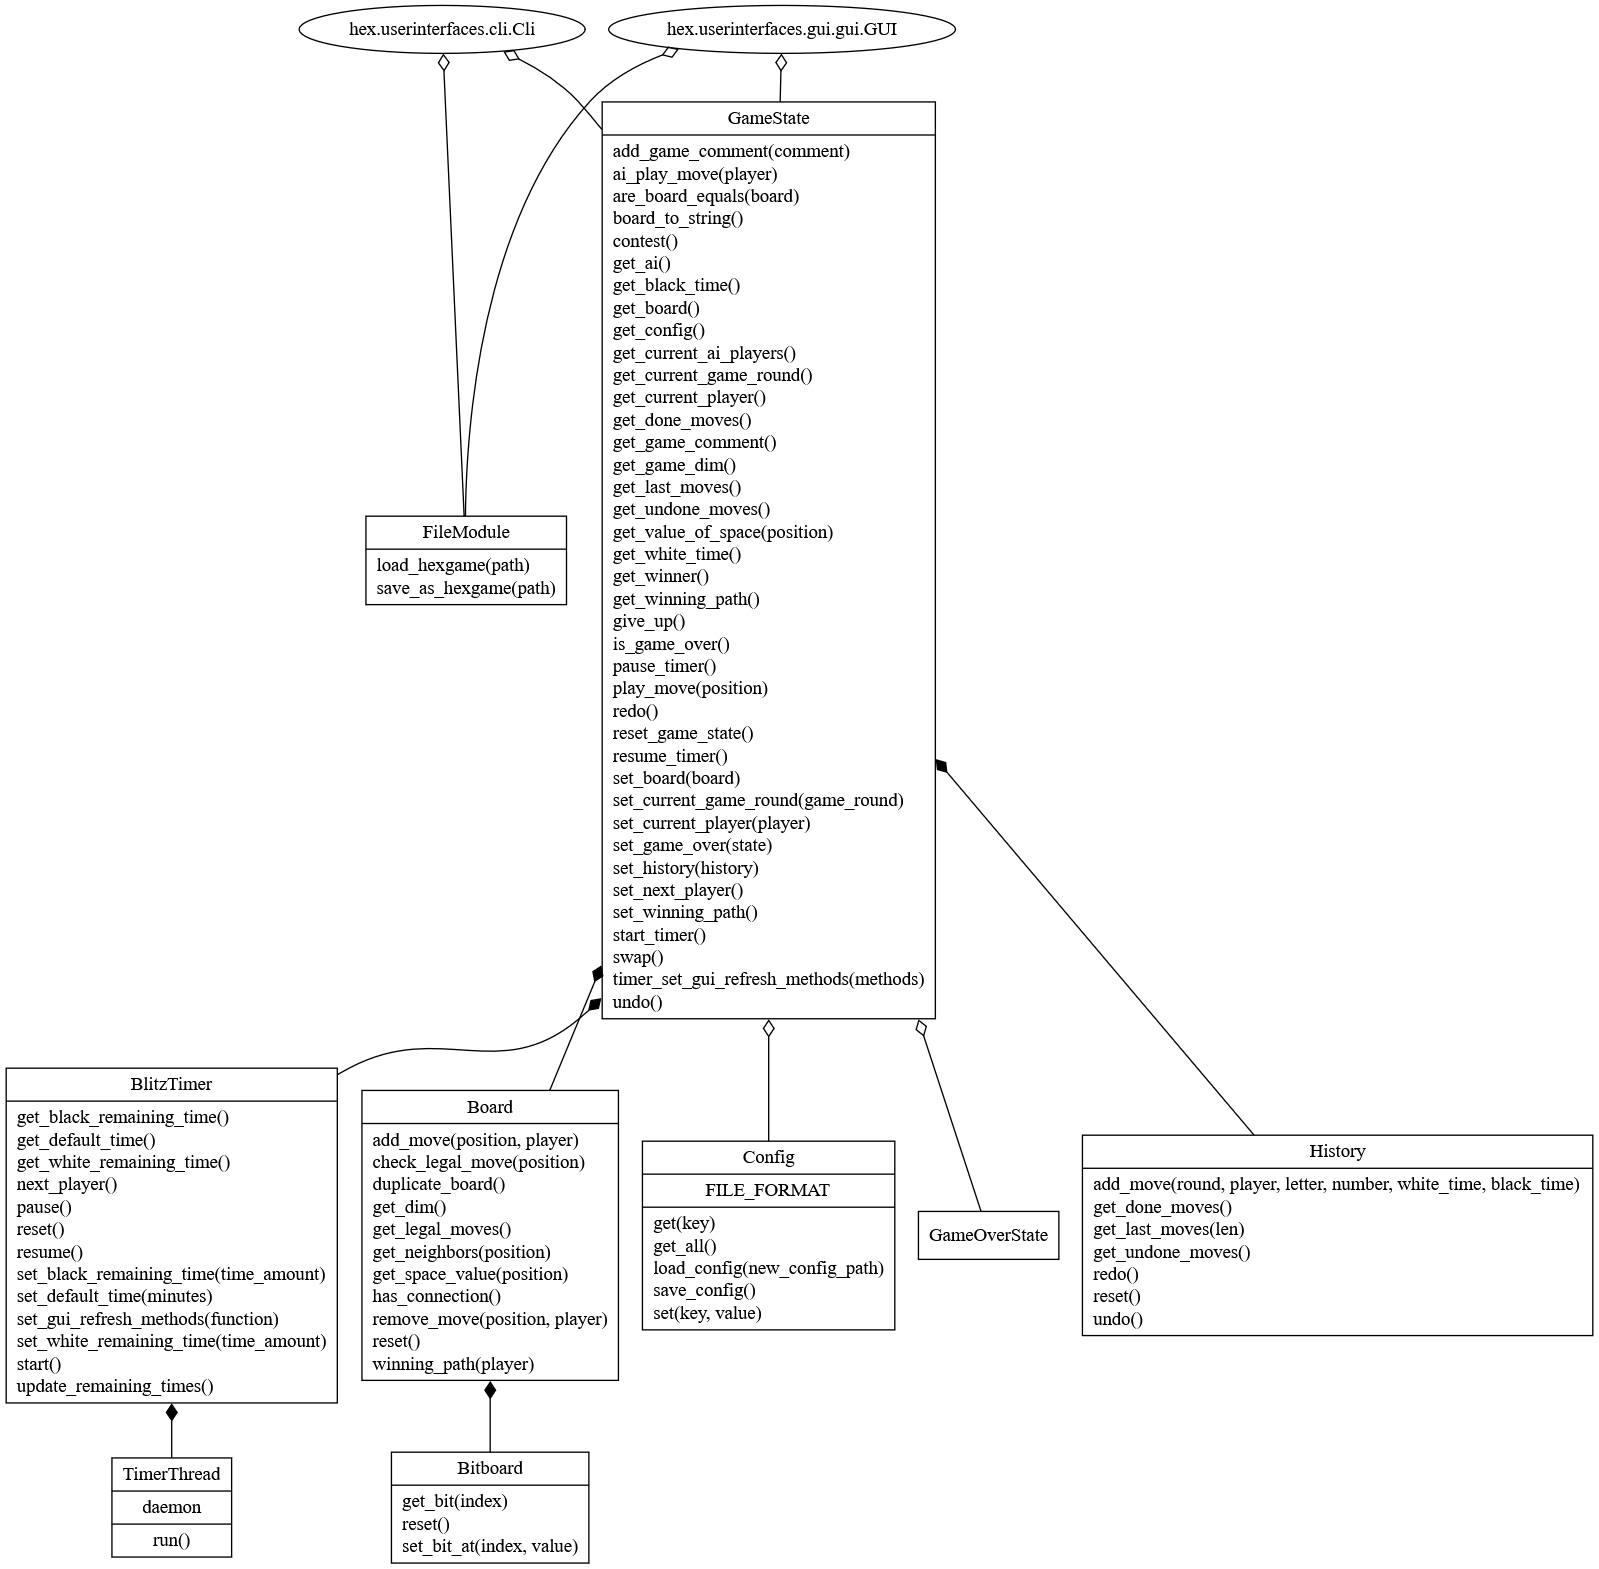
\includegraphics[width=1\linewidth]{images/UML_tools.png}
    \caption{Diagramme UML du module tools.}
    \label{fig:UML_tools}
\end{figure}

\subsection{hex.userinterfaces}

Le module du GUI créé le menu principal et l'affiche via la méthode present(). En fonction des interactions de l'utilisateur et des boutons sélectionnées, ce dernier va lui-même afficher des sous-menus ou la fenêtre de jeu. Depuis la fenêtre de jeu, il est possible d'ouvrir le menu pause et de revenir au menu principal si souhaité. Le module de gestion de fichiers est directement utilisé par les classes du CLI et du GUI (agrégation), même si ce dernier fait partie du répertoire hex.tools. Nous avons implémenté cela de la sorte à cause de problèmes de dépendances récursives.

\bigskip
\begin{figure}[H]
    \centering
    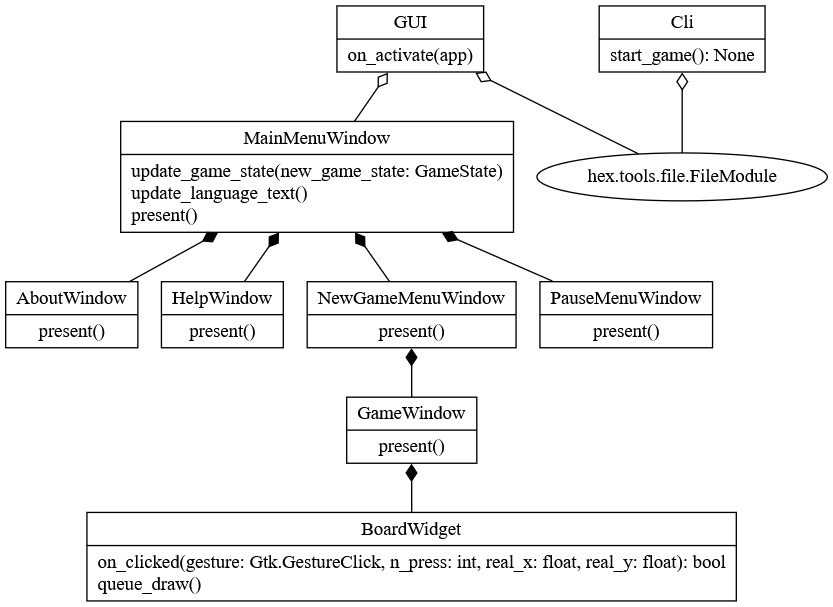
\includegraphics[width=.75\linewidth]{images/UML_userinterfaces.png}
    \caption{Diagramme UML du module userinterfaces.}
    \label{fig:UML_userinterfaces}
\end{figure}

\subsection{hex.ai}

La classe “AI Module” (hex/ai/ai.py ligne 23) contient pour chaque joueur un objet heuristique, un objet algorithme d’exploration, ainsi que les paramètres utiles à la configuration des joueurs. Elle contient aussi le temps maximal de réflexion en seconde sous la forme d’un flottant, la profondeur maximale de l’arbre de recherche sous la forme d’un entier, et les joueurs artificiels actuels sous la forme d’un tableau d’entier.

\bigskip
Un objet de type heuristique contient une fonction evaluate(board: Board, player: int) qui renvoie un entier décrivant le plateau donné en paramètre selon le point de vue du joueur passé en paramètre.

\bigskip
Un objet de type algorithme d’exploration a comme attribut un objet heuristique, une profondeur maximale sous forme d’entier, et une limite de temps en flottant. Il contient une méthode get\_move(board: Board, player: int) retournant un coup légal pour le plateau passé en paramètre.

\bigskip
Pour rendre le tout modulable et maintenable dans le futur, il a fallu rendre l’ajout d'algorithmes de décision et d’heuristiques le plus simple possible. Chaque algorithme de décision et heuristique hérite respectivement de la classe “Exploration algorithm” (hex/ai/exploration\_algorithm.py) et “Heuristic” (hex/ai/ai\_heuristic.py), jouant le rôle de pattern. Chaque algorithme doit donc implémenter une fonction get\_move(player: int, board: Board) qui renvoie un coup légal, et chaque heuristique doit implémenter une fonction evaluate(self, player: int, board: Board) qui renvoie un entier.

\bigskip
Pour ajouter une heuristique ou un algorithme d’exploration, il suffit alors d'ajouter un fichier héritant de la bonne classe (Heuristic ou Exploration algorithm) et ajouter une chaîne de caractères associée à cet algorithme dans les fonctions suivante:
\begin{itemize}
    \item si heuristique: set\_heuristic\_from\_string(heuristic: str, player: int)
    \item si algorithme d’exploration: set\_exploration\_algorithm\_from\_string(exploration\_algorithm: str, player: int) 
\end{itemize}

\bigskip
\begin{figure}[H]
    \centering
    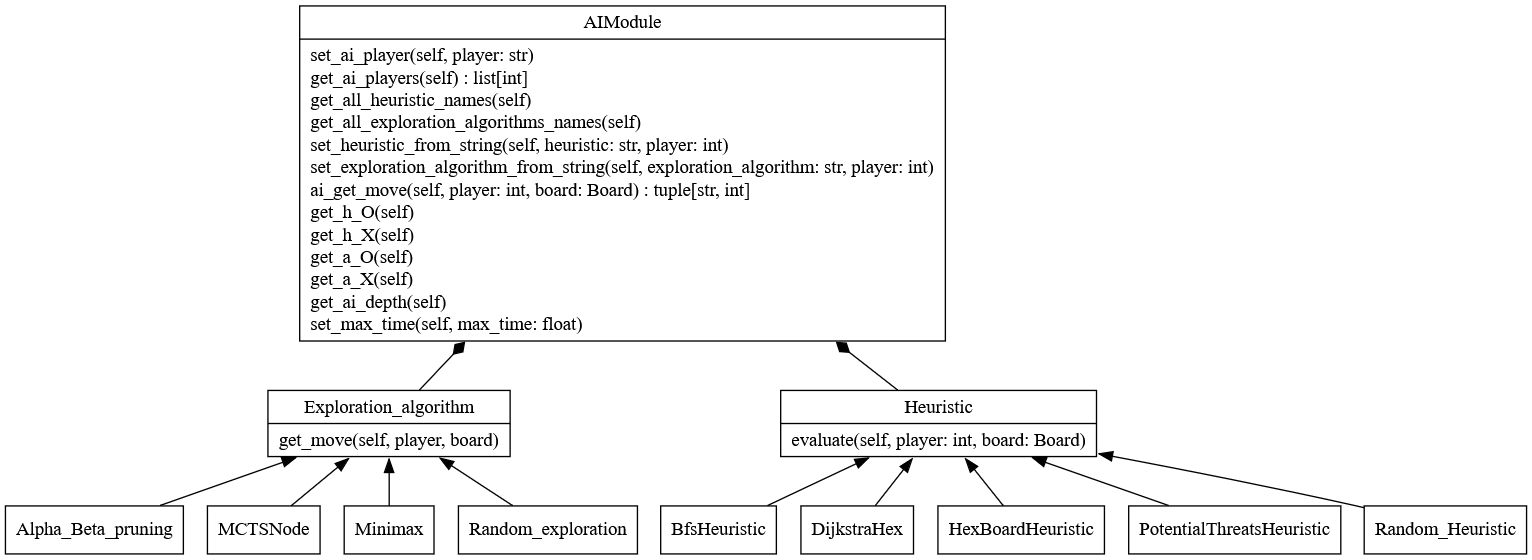
\includegraphics[width=1\linewidth]{images/UML_AI.png}
    \caption{Diagramme UML du module IA.}
    \label{fig:UML_AI}
\end{figure}

\newpage
\section{Implémentation}

Cette section regroupe les détails d'implémentation de la plupart des fonctionnalités principales de notre programme. D'autres détails sur des parties trop longues et/ou moins importantes sont disponibles en annexe \ref{annexe-impl}.
\subsection{Outils d'analyse et de formatage statique}

La qualité du code a en partie été améliorée par des outils d’analyse statique tels que \textbf{pylint} et \textbf{mypy}. Un grand nombre de défauts a pu être corrigé par pylint, mais par manque de temps, il en reste encore une certaine quantité.

\bigskip
L’outil mypy a permis de mieux annoter les types d’une grande partie de nos variables. Cependant, il reste des erreurs liées à la variable globale d’internationalisation (cf. \ref{impl-internationalisation}) qui n’est pas reconnue par mypy. Les autres erreurs correspondent à la manière dont est implémentée la configuration (cf.  \ref{impl-config}). En effet, sa méthode get renvoie une valeur qui peut prendre plusieurs types. Comme mypy ne peut pas prédire le type de retour, il rapporte beaucoup d'erreurs.

\bigskip
La commande “\textbf{autopep8} –in-line –aggressive –aggressive” a été appliquée sur chaque fichier python de notre projet afin de les formater automatiquement au style PEP8.

\bigskip
Une librairie de profiling \textbf{cProfile} nous a permis de détecter (bien que trop tard) la cause de la lenteur des IA. En enregistrant les temps d’exécution de chaque fonction, nous avons pu constater que l’algorithme de détection de fin de partie prend environ 80\% du temps d’exécution (cf. \ref{perf}).

\subsection{Gestion des options}

La gestion des options a été faite par le module argparse. Pour utiliser argparse, on doit créer un objet “ArgumentParser” qui sera le centre de l'implémentation. Il a besoin des arguments entrés en ligne de commande qu'il va interpréter. Pour que le parser interprète les différentes options, elles sont ajoutées à l’aide de la méthode “add\_argument”. Cette méthode permet plusieurs choses, tel que définir des valeurs obligatoires ou optionnelles grâce a “Choice”, attribuer des types spécifiques (str, int ...) avec “type” ou spécifier des valeurs par défaut avec “default”. Une ligne pour ajouter une option ressemble donc à ceci : parser.add\_argument(‘--size’, type=int,’ choice=[10,11,12], default=11,help=”option size”)

\bigskip
L'option -help permet à l'utilisateur d'afficher la documentation d'aide du programme qui inclut la description des options. Celle-ci est formée grâce à tous les paramètres ”help” de chaque option. Pour tester argparse, il suffit de créer une instance de ArgumentParser et de lui fournir les options voulues, puis faire des assertions sur les sorties attendues.

\bigskip
Après avoir rempli toutes les options, parser.py envoie les arguments entrées par l’utilisateur vers la configuration du jeu pour écraser ceux par défaut.

\subsection{Configuration} \label{impl-config}

Le module de configuration repose principalement sur le module python configparser, permettant de gérer facilement des fichiers au format INI. Au lancement du programme, la classe Config est instanciée avec, en paramètre, un chemin vers un fichier de configuration. Si ce fichier est valide, la configuration est stockée dans un objet de type configparser.ConfigParser. Si l’utilisateur change des options via la ligne de commande, le parser se chargera de modifier la configuration qui lui est donnée grâce à la méthode set(key, value). Le fichier de configuration étant organisé en sections (Game, AI, Dev), cette méthode détermine automatiquement la section contenant la clé de l’appelant, avant de modifier sa valeur.

\bigskip
Le module configparser propose des méthodes comme getint ou getboolean pour récupérer des valeurs directement converties comme le fait actuellement la méthode get. Cependant, nous avons fait le choix de créer une méthode \_convert\_type, ce qui nous permet de vérifier si la valeur attendue possède le bon type dès l’initialisation de la classe grâce au dictionnaire \_EXPECTED\_TYPES.

\bigskip
Son fichier de test utilise pytest.mark.parametrize avec différents fichiers de configuration, valides ou non selon le cas à tester. Les tests vérifient la validité du fichier de configuration, le type des valeurs renvoyées par get(), la modification d’une clé avec une valeur valide puis invalide dans set(), etc.

\subsection{Plateau et coups}

Le plateau est implémenté par la classe Board. Elle contient sa dimension, un bitboard pour chaque joueur et des méthodes pour le réinitialiser et ajouter, retirer et vérifier des coups à jouer. Elle possède aussi une référence vers les modules contenant les algorithmes de détection de connexion et de recherche du chemin gagnant. 

\bigskip
Un coup est représenté soit par un entier (la position du bit dans le bitboard) soit par un couple/tuple d’un caractère et d’un entier. Étant donné qu’il n’y a pas de classe représentant un coup (cf. critique \ref{crit-move}), deux méthodes translate et reverse\_translate sont nécessaires afin de passer du couple vers l’entier (indice du bitboard) et inversement lorsque nécessaire.

\bigskip
Les tests de cette classe consistent à tester toutes les positions légales pour chaque taille de plateau pour vérifier le comportement normal, ainsi que des positions aux limites, hors du plateau et incorrectes pour vérifier la levée d’erreurs.

\subsection{Fin de partie}

À chaque fois qu'un coup est joué, GameState met à jour l'état de fin de partie du jeu en l'associant a une valeur de l'enum GameOverState et, selon cet état, cherche le chemin gagnant. L’algorithme de détection de connexion est spécifié dans la partie algorithmes (\ref{algo-bpr}). Celui de la recherche d’un chemin gagnant est implémenté à l’aide d’un parcours en profondeur qui a un ordre de parcours et une priorité sur les voisins différente selon le joueur gagnant. Cet algorithme a été choisi pour sa simplicité, mais il n’est pas le plus adapté au problème et n’utilise pas les calculs sur bits que proposent les bitboards (cf. critique \ref{crit-algo-win-search}). Les comportements des deux algorithmes sont testés sur des plateaux connus à l’avance.

\subsection{Gestion des fichiers} \label{impl-fichier}

\begin{enumerate}
    \item Chargement de partie de jeu:
        Le chargement peut s’opérer via la commande load <chemin> ou en argument lorsque l’on lance le programme via l’option -l <chemin>. Avant qu’un fichier puisse charger une partie, il va subir une batterie de tests :
        \begin{itemize}
            \item On vérifie que l'extension correspond à hexgame.
            \item On vérifie que toutes les valeurs inscrites sur le plateau sont légales.
            \item On vérifie que toutes les valeurs inscrites sur l’historique sont légales.
            \item On vérifie que l’historique et le plateau correspondent.
        \end{itemize}
        Il suffit enfin de jouer tous les coups lus dans le fichier pour obtenir l'état du jeu correspondant.

    \item Sauvegarde de partie de jeu:
        La sauvegarde se fait uniquement durant d’une partie en utilisant la commande save <chemin>. On va traduire différentes informations du jeu sous la forme de chaînes de caractères. Chacune des informations occupe des sections dans le fichier, séparées par le symbole ‘\#’.
	    On écrit ensuite les différentes chaînes de caractère obtenues contenant:
        \begin{itemize}
            \item Le plateau courant.
            \item Le prochain joueur à jouer.
            \item Le numéro du tour en cours.
            \item L’historique de la partie.
            \item La dimension du plateau.
        \end{itemize}
\end{enumerate}

\bigskip
\begin{lstlisting}[style = save]
#
O.XO.O
..OOX.
XX.O..
.XXOO.
..XX.X
O..O..

#
Next player to play : 1
#
Current game round : 10
#
1. Oa1|Xc4
2. Of1|Xd5
3. Od2|Xb4
4. Oc2|Xb3
5. Od1|Xe2
6. Od3|Xc5
7. Od4|Xa3
8. Od6|Xf5
9. Oa6|Xc1
10. Oe4|
#
Game dimension is : 6
#
\end{lstlisting}
Exemple d'un fichier de sauvegarde.

\subsection{Mode blitz}

La classe BlitzTimer possède les attributs et méthodes nécessaires à l’écoulement du temps et à la gestion de l’effet du chronomètre. Les temps restants sont représentés par deux floats \_\_w\_remaining\_time et \_\_b\_remaining\_time (réinitialisables au temps par défaut \_\_default\_time)

\bigskip
Après que le CLI ou le GUI aient fini de charger, si l’option blitz est spécifiée, la méthode start() du timer est appelée. Cela démarre un thread qui retire du temps au chronomètre du joueur courant, puis prend une mesure intermédiaire qui sera utilisée pour la différence suivante. Il est aussi possible de lui donner le rôle de rafraîchir l’affichage du temps grâce à set\_refresh\_functions(), ou encore de mettre en pause le chronomètre, ce qui annule le thread et le détruit (car lancer deux fois le même thread n’est pas possible). C’est pour cela qu’il faut appeler la méthode resume() qui reprend une mesure intermédiaire et recrée et lance un nouveau thread. 

\bigskip
Le choix d’un thread pour servir de chronomètre s’explique par la volonté d’avoir un affichage du temps restant en temps réel en mode GUI.

\bigskip
Une fois que l’un des chronomètres expire, le thread met à jour l’état de fin de partie du jeu, appelle la fonction de rafraîchissement de l’affichage, envoie le signal SIGUSR1 et s’arrête. Le signal est utilisé pour lever une exception InterruptedError afin d’arrêter l’appel système qui attend l’entrée de l’utilisateur en mode CLI. Le signal est normalement masqué pendant toute l’exécution du programme, sauf lorsque l’entrée de l’utilisateur est attendue.

\bigskip
Comme Python possède (avant Python 3.13) un verrou global de l’interpréteur (GIL : global interpreter lock), les threads ne s’exécutent pas en parallèle, rendant la nécessité de verrous plus ambiguë. Cela affecte aussi les tests de cette classe. En effet, les fonctionnalités de cette classe sont testées sur des temps courts (environ deux secondes). Combiné avec des sleep, cela résulte en des tests qui ont un comportement assez instable (cf. critique \ref{crit-blitz}).

\subsection{Mode IA}

L’objectif du mode IA est d’implémenter un joueur artificiel remplaçant un ou les deux joueurs. Pour faciliter son implémentation au sein du projet, il suffit d’appeler la fonction ai\_get\_move( player: int, board: Board) (hex/ai/ai.py ligne 196) pour récupérer un coup légal, calculé par le module en fonction du joueur selon les paramètres définis dans la configuration.

\bigskip
Pour interagir avec le module (c'est-à-dire changer l’heuristique ou l’algorithme d’exploration/décision pour chaque joueur) ou changer les paramètres globaux au deux joueurs  (c'est-à-dire la profondeur maximale des arbres de recherches, le temps de réflexion maximal et les joueurs artificiels courants), on passe par des setters. Pour les heuristiques et les algorithmes d’exploration, on passe une chaîne de caractères, et si cette dernière est associée à un algorithme/heuristique, alors on attribue cet algorithme/heuristique au joueur demandé, sinon l’exploration aléatoire est attribuée à ce joueur.

\subsection{Interface en lignes de commande}

\bigskip
\begin{figure}[H]
    \centering
    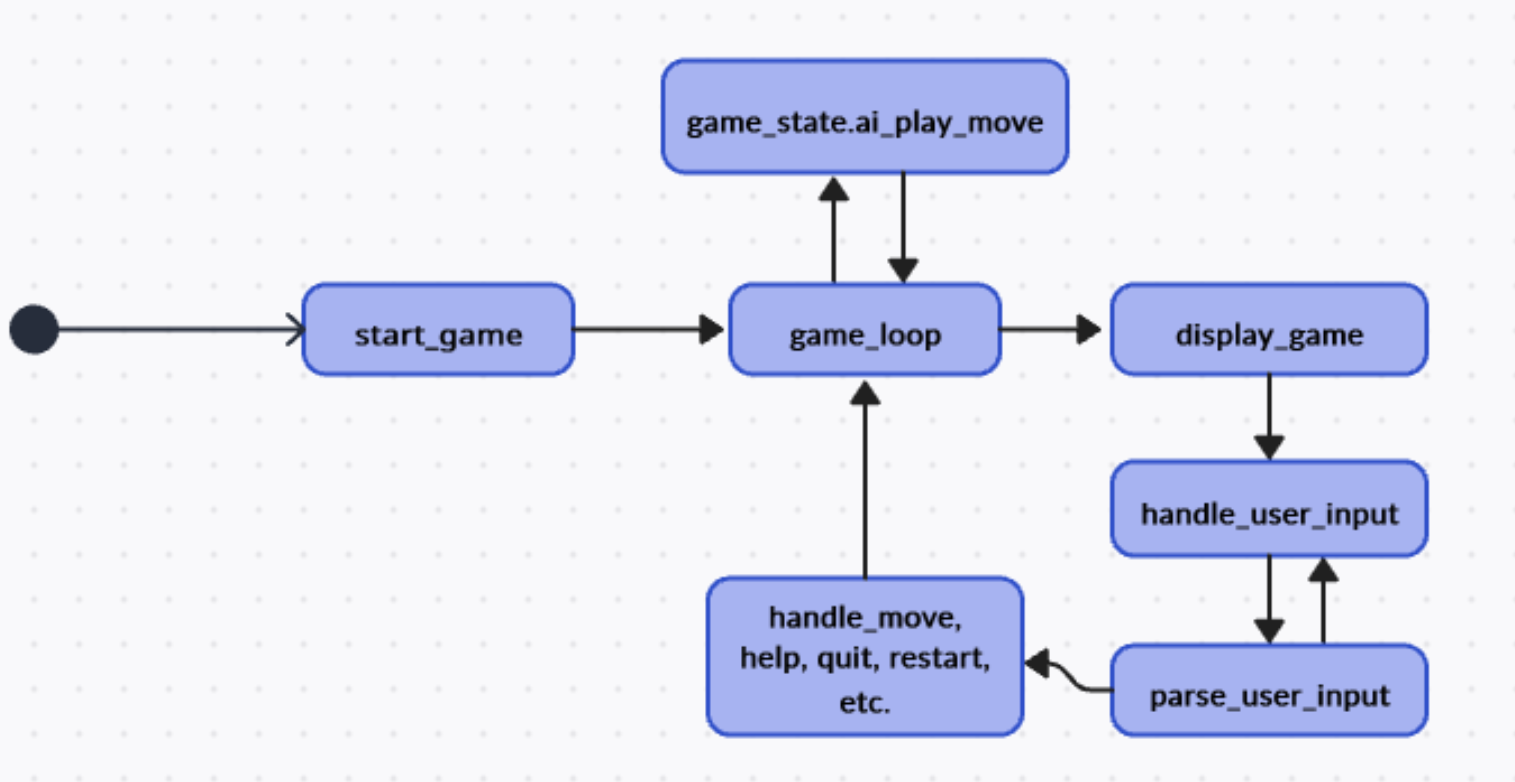
\includegraphics[width=.75\linewidth]{images/cli.png}
    \caption{Automate des interactions du CLI.}
    \label{fig:cli}
\end{figure}

L'automate représenté sur la figure \ref{fig:cli} montre le fonctionnement simplifié et le cheminement entre les différentes méthodes du module du CLI :
\begin{itemize}
    \item \textit{start\_game} est la seule méthode publique de cette classe, pouvant donc être appelée depuis un autre module (typiquement au lancement du programme).
    \item La boucle de jeu se fait via \textit{game\_loop},  de manière “récursive” et non pas avec un “while” ou tout autre type de boucle. Cette méthode va mettre à jour l’affichage (\textit{display\_game}) avant de faire appel à \textit{handle\_user\_input}.
    \item \textit{handle\_user\_input} va demander une entrée à l’utilisateur depuis le terminal avant de la faire passer à la méthode \textit{parse\_user\_input}.
    \item \textit{parse\_user\_input} va analyser (parser) cette entrée, puis va refaire appel à \textit{handle\_user\_input} si cette dernière est invalide, ou sinon faire appel à la méthode correspondant à l’action reconnue (par exemple \textit{handle\_move} si l’entrée est “a1”, qui va essayer de jouer ce coup). Le parsing est fait via des méthodes auxiliaires qui reconnaissent chacune une action spécifique. Par exemple, \textit{check\_user\_input\_display} renvoie True si l’entrée correspond à l’action de quitter le programme, sinon False.
    \item Enfin, après chaque action, on refait appel à game\_loop, qui répète ce processus.
\end{itemize}
Il est évidemment nécessaire de faire certaines vérifications au long de cet algorithme pour prendre en compte différents cas (fin de partie, action requise de l’IA, swap, etc.). Aussi, il existe une méthode \textit{confirm} servant simplement à demander une confirmation en cas d'action “critique” (quit, restart, etc.).

\bigskip
Ce module servant à l’affichage, il agrège une instance de GameState, dont il fait appel pour la plupart des actions afin que l’état courant du jeu soit modifié et mémorisé, et dont il se sert pour mettre à jour l’affichage de façon adéquate.

\subsection{Interface graphique}

Les fonctionnalités associées aux besoins F46, F47 et F48 sont réparties dans différentes fenêtres. Les menus File, Game, et About ne sont donc pas implémentés via des menus déroulants mais des fenêtres.

\bigskip
Chaque fenêtre prend en argument une instance de GameState, et les fenêtres contenant un bouton Retour prennent en second argument une référence vers la fenêtre précédente.

\bigskip
La fenêtre de jeu est différente car elle interagit et dépend de l'état du jeu représenté par GameState. En plus d'afficher des informations et de proposer des interactions avec des boutons, elle possède un widget personnalisé nommé BoardWidget qui représente l’affichage du plateau de jeu. Ce widget utilise un moteur de rendu pour générer l'affichage du tableau et gère aussi le fait de pouvoir jouer sur un hexagone avec le clic de la souris.

\bigskip
Les détails d'implémentations et des figures des différents menus sont disponibles en annexe \ref{annexe-gui}, ainsi que ceux de l'affichage du plateau et de la détection de clic en annexe \ref{annexe-gui-board}.

\newpage
\section{Performances et Limitations}

\subsection{Performances en temps}  \label{perf}

Les trois figures \ref{fig:has_conn_time}, \ref{fig:gui_time} et \ref{fig:alpha_time} montrent le rapport quadratique entre la dimension du plateau et les différents algorithmes principaux du programme. Nous remarquons aussi dans la figure \ref{fig:gui_time} un pic dans le temps de rafraîchissement de l'affichage de la fenêtre de jeu lorsque le plateau a une dimension de 16. La raison de ce ralentissement nous est inconnu.

\bigskip
\begin{figure}[H]
    \centering
    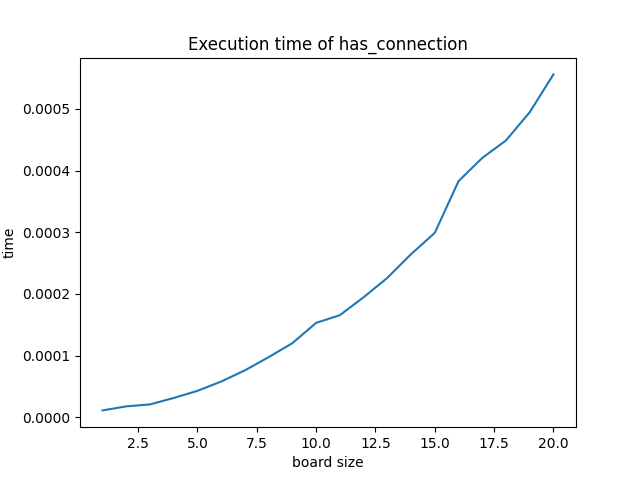
\includegraphics[width=.55\linewidth]{images/has_connection_time.png}
    \caption{Temps d'exécution en secondes de la méthode has\_connection sur chaque taille de plateau (3 expériences). On observe un début de parabole montrant bien la complexité en O(dim²) de l'algorithme.}
    \label{fig:has_conn_time}
\end{figure}

\bigskip
\begin{figure}[H]
    \centering
    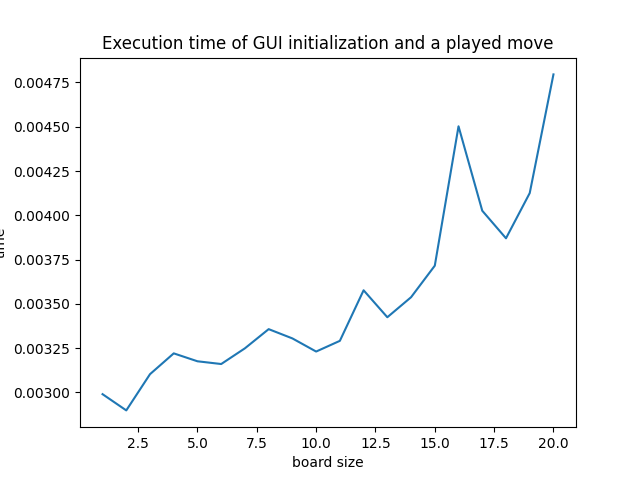
\includegraphics[width=.55\linewidth]{images/gui_time.png}
    \caption{Temps d'exécution en secondes de l'initialisation du GUI suivi d'un coup joué pour déclencher le rafraîchissement de l'affichage sur chaque taille de plateau (3 expériences). Le temps d'exécution de l'initialisation étant égale entre chaque taille de plateau, il a été décidé de rajouter le rafraîchissement de l'affichage. Cela montre que la dimension du plateau a une influence sur le temps d'affichage.}
    \label{fig:gui_time}
\end{figure}

\bigskip
\begin{figure}[H]
    \centering
    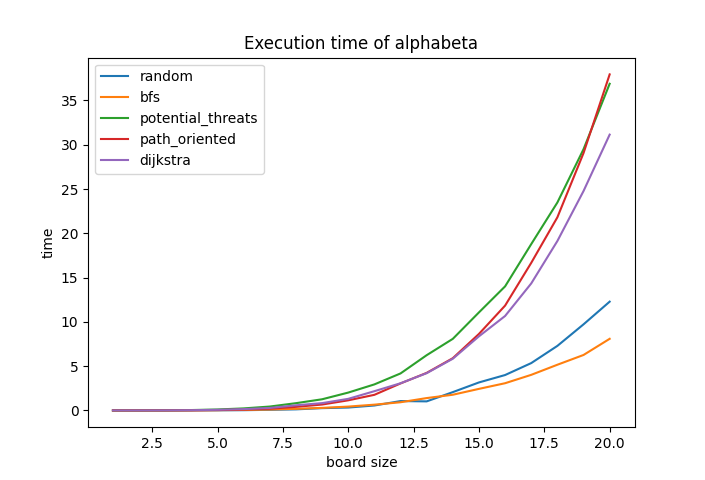
\includegraphics[width=.7\linewidth]{images/alpha_beta_time.png}
    \caption{Temps d'exécution en secondes de l'exploration Alpha-Beta pour une profondeur maximale de 2, pour chaque heuristique et chaque taille de plateau (3 expériences). (Random peut être plus lent quand il y a moins de branches à élaguer.)}
    \label{fig:alpha_time}
\end{figure}

Les figures \ref{fig:alpha-prof} et \ref{fig:mcts-prof} montrent que l'algorithme de détection de connexion prend environ 80\% du temps de réflexion des IA. Nous remarquons aussi que le temps d'exécution de la conversion des bitboards vers la structure utilisée pour la réduction est similaire à la réduction en elle même. Il serait pertinent d'utiliser directement la structure durant tout le programme pour diviser par deux le temps d'exécution de la détection de connexion.

\bigskip
\begin{figure}[H]
    \centering
    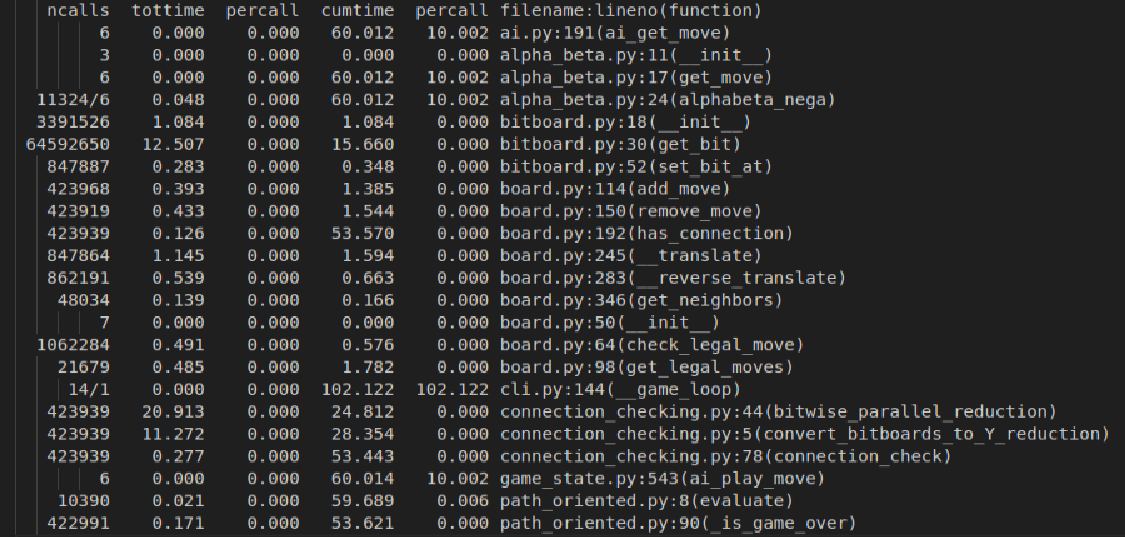
\includegraphics[width=.85\linewidth]{images/alpha_beta_prof.png}
    \caption{Tableau obtenu après l'utilisation de cProfile sur l'exécution de notre programme pendant six tours sur un tableau de taille 7 avec Alpha-Beta en tant qu'opposant. 53.5 secondes parmi les 60 secondes du temps de réflexion de l'IA (ai\_get\_move) sont consacrées à la détection de connexion (is\_game\_over).}
    \label{fig:alpha-prof}
\end{figure}

\bigskip
\begin{figure}[H]
    \centering
    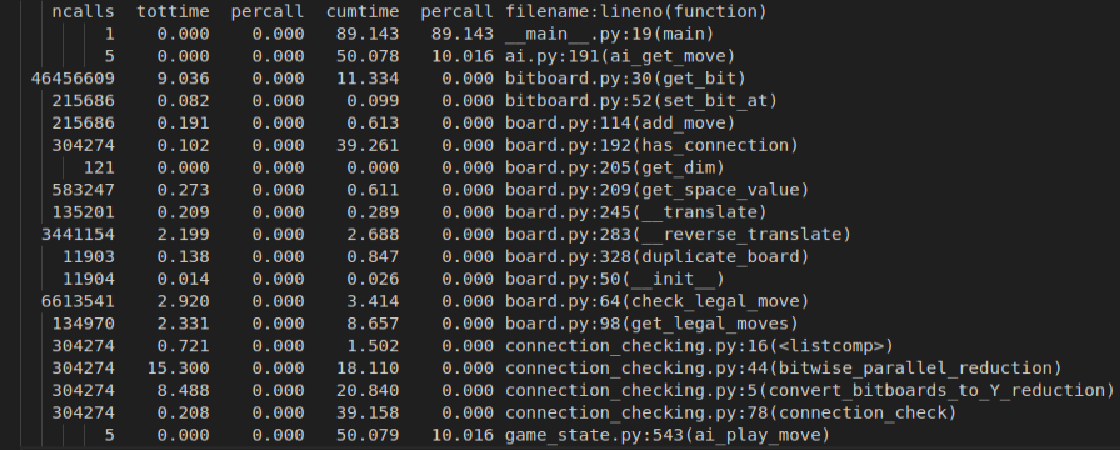
\includegraphics[width=.85\linewidth]{images/mcts_prof.png}
    \caption{Tableau obtenu après l'utilisation de cProfile sur l'exécution de notre programme pendant cinq tours sur un tableau de taille 7 avec mcts en tant qu'opposant. 39.2 secondes parmi les 50 secondes du temps de réflexion de l'IA (ai\_get\_move) sont consacrées à la détection de connexion (has\_connection).}
    \label{fig:mcts-prof}
\end{figure}

\subsection{Performances en jeu des IA}

\bigskip
\begin{figure}[H]
    \centering
    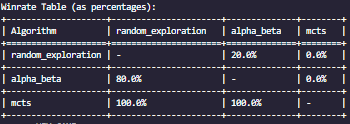
\includegraphics[width=.6\linewidth]{images/tab_ia.png}
    \caption{Tableau montrant les différents résultats des algorithmes de décisions les uns contre les autres. Paramètres : plateau de taille 4, temps de réflexion maximum de 20s, profondeur maximale de 3, heuristique Dijkstra, échantillonnage sur cinq parties, après chaque partie les algorithmes échangent de couleurs. Par souci de temps, minimax n’est pas inclus, car il renvoie les mêmes résultats qu'Alpha-Beta.\\
    Exemple de lecture : Alpha-Beta gagne 80\% du temps contre l’exploration aléatoire.}
    \label{fig:tab_ia}
\end{figure}
	
On remarque sur la figure \ref{fig:tab_ia} que MCTS (Monte Carlo Tree Search Algorithm), gagne 100\% du temps contre nos autres algorithmes. 

\bigskip
Sur des machines plus lentes, il est recommandé d’augmenter le temps de réflexion maximal. Le temps recommandé est 30 secondes pour Alpha-Beta et MCTS.

Alpha-Beta explore les coups de manière linéaire, c'est-à-dire de gauche à droite et de haut en bas. Il peut donc arriver qu'Alpha-Beta ne renvoie pas le bon coup quand le temps arrive à terme, car il n’a pas eu le temps d’explorer la totalité des coups. En pratique, sur un temps qui restreint Alpha-Beta, dépendamment de la machine, Alpha-Beta va avoir tendance à jouer dans les premières lignes du tableau.

\bigskip
Amélioration possible pour Alpha-Beta : Exécuter Alpha-Beta avec une profondeur qui varie au fur et à mesure que la partie avance car les premiers coups sont déterminés par la stratégie des heuristiques et non les coups de l’adversaire. La profondeur augmenterait petit à petit jusqu’à atteindre la profondeur maximale en fin de partie quand la complétion de chemin est plus importante et qu’il y a moins de coups possibles. Cela permettrait d’atteindre des profondeurs plus élevées sans pour autant impacter le temps de recherche.

\bigskip
De plus, on pourrait mélanger les coups parcourus de façon à placer les meilleurs coups en premier dans l’arbre de recherche, ce qui augmenterait significativement les performances d’Alpha-Beta. Cela impliquerait de concevoir une stratégie globale pour n’importe quel plateau.

\bigskip
MCTS quant à lui simule des parties aléatoires à partir de coups aléatoires au départ, puis privilégie les coups avec les meilleurs résultats. Il faut savoir que, dans ce projet, MCTS est paramétré avec un grand nombre de simulations, ce qui va avoir pour conséquence d’utiliser la totalité du temps à sa disposition pour prédire le meilleur coup possible. Ses performances sont alors grandement impactées par la machine qui exécute le programme.

\bigskip
\begin{figure}[H]
    \centering
    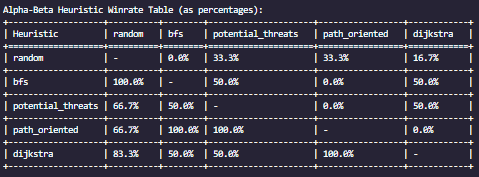
\includegraphics[width=.7\linewidth]{images/tab_heuristiques.png}
    \caption{Tableau montrant les différents résultats des heuristiques les unes contre les autres. Paramètres : plateau de taille 6, temps de réflexion maximum de 20s, profondeur maximale de 3, échantillonnage sur six parties, après chaque partie les algorithmes échangent de couleur.}
    \label{fig:tab_heur}
\end{figure}

On remarque sur la figure \ref{fig:tab_heur} que l’heuristique path\_oriented (cf. \ref{path_oritented}) montre les meilleurs résultats, ce qui est en accord avec l’objectif de l’heuristique qui intègre des principes spécifiques au jeu de Hex. Néanmoins, on note que l’heuristique path\_oriented a perdu la totalité des parties contre l’heuristique dijkstra (cf. \ref{algo-dijkstra}), ce que l’on peut interpréter comme une richesse des stratégies et qui signifie qu’il y a des stratégies qui marchent particulièrement bien les unes contre les autres.

\bigskip
Contre un joueur artificiel aléatoire, toutes les heuristiques gagnent plus de 50\% du temps, on a donc une certaine réflexion qui se dégage des stratégies de jeu.

\newpage
\section{Critiques et Perspectives} \label{critiques}

Notre jeu fonctionne parfaitement en joueur contre joueur. L'interface en lignes de commande et l'interface graphique permettent d'offrir des interactions à l'utilisateur et de les gérer. Il peut sauvegarder et charger une partie, jouer contre une IA, utiliser les options en lignes de commande et depuis le menu de l'interface graphique. Cependant, il existe toujours des perspectives pour rendre ce projet meilleur. Notamment sur la détection de la fin de partie \ref{crit-connec}.

\subsection{Affichage et interactions avec le plateau dans le GUI} \label{crit-gui-board}

L’implémentation de l’affichage du plateau utilise des carrés qui contiennent chacun l’image d’un hexagone. Étant donné qu’entre les lignes du plateau, les hexagones se touchent au niveau de leurs diagonales, ces carrés se chevauchent. Cela est un problème, car la fonction utilisée pour vérifier qu’un clic de la souris se trouve dans un hexagone nécessite le carré dans lequel se trouve l’hexagone. Cela oblige à vérifier le clic dans les deux carrés au-dessus ainsi que les deux se trouvant en dessous. De plus, l’utilisation de carrés pour stocker les hexagones fait que ce ne sont pas des hexagones réguliers (côtés de même longueur). Ces deux manières de faire ne sont pas un standard, complexifient le traitement du clic de la souris et pourraient nuire à de futures améliorations. Pour régler ceci, il faudrait reprendre l’implémentation en utilisant des hexagones réguliers et un système de grille et de coordonnées comme décrit dans cette compilation de données sur les grilles hexagonales par Amit Patel \cite{AP}, qui s'est à la base inspiré des travaux de Ed Luczak et Azriel Rosenfeld \cite{LuczakRos76}. Cela permettrait d’instantanément savoir dans quel hexagone le clic se trouve.

\subsection{Ajout d’un type Move} \label{crit-move}

Les coups du jeu de hex dans notre programme sont représentés de deux manières différentes : soit par un entier (position dans le bitboard), soit par un couple composé d’un caractère (colonne) et d’un entier (ligne). Des méthodes de conversion sont donc nécessaires, car les bitboards utilisent des entiers alors que le reste du programme utilise le couple. Pour régler cette ambiguïté, il serait pertinent de créer une classe Move qui représente les coups du jeu. Elle pourrait être initialisée avec soit un entier, soit un couple caractère/entier et permettrait de récupérer les deux formes selon la situation, éliminant la nécessité de convertir.

\subsection{Tests de blitztimer} \label{crit-blitz}

Les tests vérifiant le comportement de la classe BlitzTimer ont occasionnellement des résultats indéterminés. Les temps des chronomètres sont fixés à deux secondes pour ne pas que les tests prennent trop de temps, et des appels à time.sleep sont utilisés pour faire passer le temps. Certaines assertions peuvent ne pas passer, car le thread met trop de temps à se réveiller. Dans ce cas, il se peut que le temps du timer soit entièrement écoulé à des moments inattendus, ou que le thread mette trop de temps à s’endormir et enregistre donc des valeurs après que le thread principal ai fait la mesure pour le test.

\bigskip
Par exemple, dans test\_pause\_and\_resume, le thread principal demande au timer de se mettre en pause. Puis le thread principal lit le temps restant et le stocke dans une première mesure. Le thread timer peut se réveiller juste après la demande de pause. Dans ce cas, les assertions passent correctement. Dans le cas contraire, s'il se réveille après la mesure, il va écrire un nouveau temps et s’arrêter. Lorsqu'une deuxième mesure sera effectuée pour vérifier que le timer s’est bien arrêté et que la valeur du temps restant n’a pas changé, il se peut que les deux mesures soient différentes et que l’assertion ne passe pas.

\bigskip
Durant le déroulement normal du programme, l’ordre des écritures et lectures n’est pas important. Le fait que les threads fassent les choses dans le mauvais ordre n’est donc pas un problème, car avec le GIL (Global Interpreter Lock), les threads ne s’exécutent pas en parallèles et il n'y a donc pas de problème de lectures et écritures concurrentes. Cependant, durant les tests, il serait une bonne idée de rajouter des verrous pour éviter des écritures non voulues.

\subsection{Recherche du chemin gagnant} \label{crit-algo-win-search}

L’algorithme de parcours en profondeur, ou en tout cas la manière dont le chemin est renvoyé, n’est pas le plus adapté pour trouver le chemin gagnant. En effet, il se peut que des cases en trop fassent partie du chemin renvoyé. Dans l’idéal, le chemin le plus court devrait être affiché. Des algorithmes comme Dijkstra \cite{dijk} ou A* \cite{4082128} avec une heuristique adaptée seraient de meilleures solutions, même si elles nécessiteraient peut-être d’ajouter des structures de données ou de convertir les bitboards en une structure plus adaptée.

\subsection{Détection de connexion} \label{crit-connec}
L’algorithme BPR utilisé pour la détection de connexion (cf. algorithme \ref{algo-bpr}) est un problème lorsqu’il devient nécessaire de l’appeler de nombreuses fois. En effet, dans l'article \cite{browne12}, il est expliqué que BPR est le meilleur algorithme lorsqu’il s’agit de savoir si une partie quelconque est gagnée, car son temps de calcul dépend seulement de la taille de l’entrée (cf. Figure \ref{fig:Browne-per-game}). Cependant, il n’est pas le meilleur s'il est appliqué à chaque coup durant le déroulement d’une partie entière (cf. Figure \ref{fig:Browne-per-move}). Des algorithmes de recherche par union sont deux fois plus rapides en moyenne, car plus efficaces en début de partie.

\bigskip
\begin{figure}[H]
    \centering
    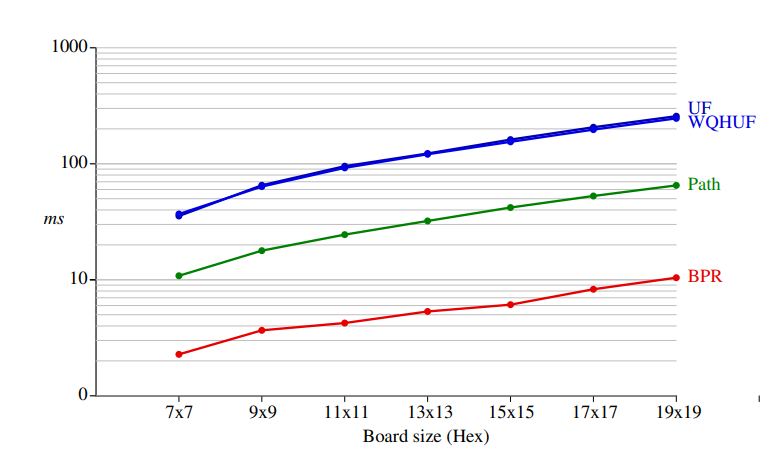
\includegraphics[width=.7\linewidth]{images/per_game_bpr.png}
    \caption{Millisecondes pour 10000 parties avec une vérification par partie, dans le jeu de Hex (Figure de \cite{browne12}). L'échelle étant logarithmique, il est évident que BPR est l'algorithme le plus efficace lorsqu'il n'est utilisé qu'une seule fois pour vérifier une partie quelconque.}
    \label{fig:Browne-per-game}
\end{figure}

\bigskip
\begin{figure}[H]
    \centering
    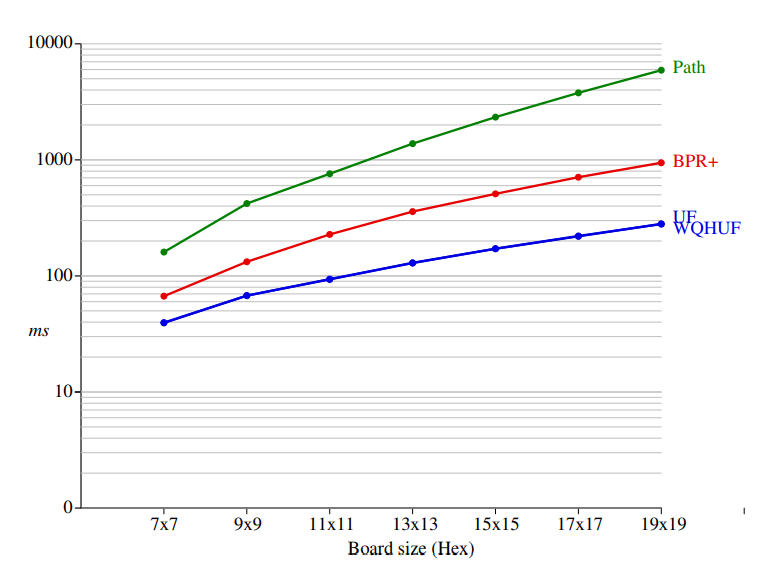
\includegraphics[width=.65\linewidth]{images/Per-move-bpr.png}
    \caption{Millisecondes pour 10000 parties avec une vérification par coup, dans le jeu de Hex (Figure de \cite{browne12}). L'échelle étant logarithmique, il est évident que BPR est moins efficace, lorsqu'il est utilisé à chaque coup joué, que Union Find ou Weighted Quick Union Find.}
    \label{fig:Browne-per-move}
\end{figure}

Cette lenteur impacte massivement nos IA et les fonctionnalités qui en dépendent (fonction du bouton ‘hint’ ralenti ce qui affiche une popup "not responding" ainsi que le mode contest), rendant le mode joueur contre IA pénible sur de grands plateaux (et chronophage). Pour avoir une difficulté satisfaisante, l’IA doit tourner plusieurs dizaines de secondes. La détection de connexion correspond en effet à 80\% du temps de recherche des IA (cf. section performances \ref{perf}).

\bigskip
Pour espérer avoir de meilleures performances, il est possible d’appeler cette détection de connexion qu’après un certain nombre de tours ou dès que le joueur forme un paterne qui pourrait être une connexion. Nous pourrions aussi représenter le plateau directement avec la structure utilisée par l'Y-réduction, divisant déjà par deux le temps d'exécution (cf. section \ref{perf}). Aussi, il serait peut-être plus pertinent de passer d’un algorithme à un autre selon l’état d’avancement de la partie. Au début, un algorithme de recherche par union serait utilisé, puis changerait pour BPR en fin de partie. Des wrappers C pourraient aussi être utilisés pour faire tourner les algorithmes importants en C, en profitant éventuellement de la parallélisation. Cela permettrait d’améliorer les performances non seulement en temps d’exécution, ce qui rendrait le jeu plus jouable contre l’IA, mais aussi en "qualité" des coups joués par l’IA MCTS qui bénéficierait de plus de simulations.

\subsection{Fichiers de sauvegarde}

Par soucis de temps, les fichiers de sauvegarde n’ont été représentés que sous la forme d’un seul format : le format hexgame (cf. \ref{impl-fichier}). Ce format est loin d’être parfait car il ne contient pas les informations qui ont été développées plus tard, tel que le module de blitz, ou la configuration de la partie.
Dans le futur, il faudrait ajouter l’information du temps de chaque coup lorsque le mode blitz est activé, ainsi que la configuration actuelle de la partie que l’on trouve dans la classe Config().

\newpage
\addcontentsline{toc}{section}{Références}
\bibliographystyle{alpha}
\bibliography{biblio}

\newpage
\appendix
\appendixpage
\addappheadtotoc

\section{Liste des besoins implémentés}
Cette liste présente les besoins qui ont été implémentés (ainsi que le seul qui n'a pas du tout été implémenté en rouge), accompagnés de leurs modifications par rapport aux spécifications.

\bigskip
\begin{itemize}
    \item \textbf{F1 : Langage de programmation}
    
Le langage de programmation choisi pour ce projet est Python 3.10.12. (Python 3.8 a été testé, mais nécessite un fichier setup.py pour l’installation, et un problème de compatibilité avec la librairie GTK a été constaté.)
    \item \textbf{F2 : Style de codage}
    \item \textbf{F3 : Langue par défaut dans le code}
    \item \textbf{F4 : Système cible}
    
    Le programme fonctionne sur Ubuntu 22.04.5 et les machines Debian du CREMI.
    \item \textbf{F5 : Documentation}

    Le manuel utilisateur se trouve dans le README.
    \item \textbf{F6 : Tests}

    Couverture de 84\%.
    \item \textbf{F7 : Bugs}
    \item \textbf{F8 : Performances}
    
    Un rapport des performances de certaines fonctions et des IA est disponible dans le README.
    \item \textbf{F9 : Build-system}
    \item \textbf{F10 : Framework de tests}
    \item \textbf{F11 : Gestion des options}
    \item \textbf{F12 : Bibliothèque graphique}
    \item \textbf{F13 : Internationalisation}
    \item \textbf{F14 : Nom de l'exécutable principal}
    \item \textbf{F15 : Usage général}
    \item \textbf{F16 : Aide en ligne de commande}
    \item \textbf{F17 : Version}
    \item \textbf{F18 : Mode verbose}
    \item \textbf{F19 : Mode debug}
    \item \textbf{F20 : Mode Blitz}
    \item \textbf{F21 : Durée du blitz}
    \item \textbf{F22 : Changement de couleur / Inversion  des joueurs}

    Au lieu de changer de couleur, le second joueur peut choisir d’écraser le coup du premier. Ceci produit le même résultat et permet de conserver sa couleur.
    \item \textbf{F23 : Taille du plateau}
    \item \textbf{F24 : Mode contest}
    \item \textbf{F25 : Mode IA}
    \item \textbf{F26 : Interface en ligne de commande}
    \item \textbf{F27 : Interface graphique}
    \item \textbf{F28 : Affichage du plateau}

    L’affichage du plateau comporte des ‘o’ et des ‘x’ au niveau des bordures pour que l’utilisateur reconnaisse plus facilement quelles sont ses deux bordures parallèles.
    \item \textbf{F29 : Notation des coups}
    \item \textbf{F30 : Représentation de l’historique}
    \item \textbf{F31 : Abandon}
    \item \textbf{F32 : Affichage des messages}
    \item \textbf{F33 : Quitter et sauvegarder une partie}

    Les temps restants du mode blitz ne sont pas sauvegardés.
    \item \textbf{F34 : Sauvegarde de l’historique}

    L’historique et le plateau sont sauvegardés ensemble. Il n’y a pas le choix de sauvegarder que le plateau ou que l’historique.
    \item \textbf{F35 : Naviguer dans l’historique}
    \item \textbf{F36 : Recommencer une partie}
    \item \textbf{F37 : Fin de partie}
    \item \textbf{F38 : Rejouer une partie}

    Charger une partie où un swap a été effectué renverra une erreur de format du fichier. De plus, charger une partie qui était en mode blitz ne restaurera pas le temps.
    \item \textbf{F39 : Format de fichier}

    Le plateau est représenté comme un rectangle au lieu d’un parallélogramme. La ligne à laquelle se situe l’erreur n’est pas affichée.
    \item \textbf{F40 : Format de l’historique}

    L’historique est attaché au fichier de sauvegarde du plateau.
    \item \textbf{F41 : Fichier de configuration}
    \item \textbf{F42 : Plateau de jeu}
    \item \textbf{F43 : Module bitboard}
    \item \textbf{F44 : État du jeu}

    Les temps restants sont stockés dans le module blitztimer qui est lui-même contenu dans l’état du jeu.
    \item \textbf{F45 : Fonctions de base}
    \item \textbf{F46 : Menu 'File'}

    Nous avons adopté une approche “plein écran” pour l'interface graphique du jeu. Les items ‘New Game’, ‘Load Game’, ‘Help’ et ‘Quit’ se trouvent dans la fenêtre ‘Main Menu’. L’item ‘Save Game’ se trouve dans le menu ‘pause’ de la fenêtre de jeu. L’item ‘Settings’ n’est pas présent. La configuration par défaut ne peut être changée qu’en éditant le fichier config.checkersrc.
    Le menu ‘Help’ affiche la configuration du jeu, les règles du jeu et des stratégies de jeu.
    \item \textbf{F47 : Menu ’Game’}

    Ces fonctionnalités sont utilisables par des boutons dans la fenêtre de jeu.
    \item \textbf{F48 : Menu ’About’}
    
    Cet item se trouve dans le menu principal.
    \item \textbf{F49 : Affichage d’une partie en cours}
    \item \textbf{F50 : Affichage des coups joués}
    \item \textbf{F51 : Configuration d’une nouvelle partie}

    L’item ‘New Game’ affiche une nouvelle fenêtre avec la configuration par défaut, que l’utilisateur peut modifier. Cette fenêtre est accessible à partir du menu principal. Il n’y a pas de menu ‘File’.
    \item \textbf{F52 : Heuristique d’évaluation de position}
    \item \textbf{F53 : Algorithme de recherche Minimax}
    \item  \textbf{F54 : $\alpha\beta$-pruning}
    \item \textcolor{red}{\textbf{NON IMPLÉMENTÉ F55 : Exploration peu profonde préliminaire}}
    \item \textbf{F56 : Monte Carlo Tree Search}
    \item \textbf{F57 : Profondeur de recherche}
    \item \textbf{F58 : Choix des heuristiques}
    
    Il est possible de choisir l’heuristique ainsi que l’algorithme de recherche pour chaque joueur.
    \item \textbf{F59 : Heuristique de fin de partie}
    \item \textbf{F60 : Temps de réflexion borné}
\end{itemize}

\section{Détails d'implémentation} \label{annexe-impl}

\subsection{Exécutable principal}

L’exécutable principal (\_\_main\_\_.py) est appelé lorsque la commande hex <options> est entrée dans le terminal. Dans un scénario classique, il initialise la configuration du jeu (par la classe Config qui lit le fichier de configuration), appelle la méthode parse\_args du module argparse.py (pour charger les options passées par l’utilisateur), initialise l’état du jeu, charge un jeu si un fichier est spécifié et lance l’interface demandée. Il gère aussi les comportements lorsque les options –version et –contest sont spécifiées. Des messages sont affichés lorsque des problèmes sont rencontrés lors de la lecture des fichiers de configuration ou de sauvegarde.

\subsection{Affichage des messages/logging (verbose et debug)}

Les options "verbose" ou "debug" sont reconnues par le parser puis écrites dans la configuration. Ensuite, pour les faire fonctionner, nous avons implémenté un fichier logger.py. Pour le logger, on doit mettre en place différents logging\_level en fonction des besoins, dans notre cas verbose et debug. Ensuite, une fonction log interprète le loglevel et le message et décide s'il doit être affiché en fonction de son log\_level. Pour afficher un message, il suffit de le placer à l'endroit souhaité, par exemple dans le fichier main\_menu\_gui.py ligne 206 pour notre code :
log(LogLevel.DEBUG, "User interaction : Contest mode")

Donc ce message s'affiche grâce à log en mode debug.

\subsection{Internationalisation} \label{impl-internationalisation}
Ce besoin a été réalisé grâce à la bibliothèque gettext comme demandé dans le cahier des charges. Gettext marche de façon particulière, il a fallu placer un bout de code pour initialiser gettext dans tous les fichiers.py qui servent à l’affichage de texte (tel que les interfaces) :

\begin{lstlisting}[style = PythonStyle]
global lang
        lang = game_state.get_config().get("language")
        language_translations = gettext.translation(
            "base", localedir="hex/userinterfaces/locales", languages=[lang])
        language_translations.install()

        global _
        _ = language_translations.gettext
\end{lstlisting}

La variable lang est utilisée pour récupérer la langue couramment utilisée par le programme. Elle appelle config pour récupérer le champ langage. Ensuite, language\_translations cherche un fichier MO (.mo) servant pour la traduction, nommé "base" depuis le chemin "localdir" avec la langue “lang”.
La variable “\_” sert à indiquer quel chaîne de caractères on souhaite traduire. Pour se faire, il faut l’ajouter avant chaque chaîne à traduire :
print(“bonjour”) → print(\_(“bonjour”))

\bigskip
Après avoir indiqué tous les textes à traduire, il faut créer un fichier PO (.po) qui indique tous les strings du fichier à traduire. Il suffit donc de les traduire dans la langue souhaitée, les mettre à la bonne place (dans /locales/<’en’ ou ‘fr’>/LC\_MESSAGES) et les compiler en MO (.mo).

\section{Implémentation du plateau dans le GUI} \label{annexe-gui-board}
\begin{enumerate}

\item \textbf{Initialisation}

L’affichage du plateau de jeu est possible grâce au widget GTK personnalisé BoardWidget du fichier board\_gui.py. Il est initialisé avec une référence à l’état du jeu et récupère la dimension du plateau depuis ce dernier. Depuis cette dimension, la dimension des carrés qui vont contenir les images des hexagones (et qui par conséquent ne sont pas des hexagones réguliers) (cf. critique \ref{crit-gui-board}) est obtenue. La hauteur et la largeur virtuelle, calculées à partir de la dimension d’un carré, et qui sont constantes par rapport à la véritable taille du widget pouvant évoluer, servent à calculer l’échelle du widget par rapport à sa taille réelle affichée. Cette valeur est stockée dans l’attribut \_\_current\_scale et est passée à la méthode scale() de snapshot à chaque rafraîchissement de l’affichage pour remettre à l’échelle les axes des coordonnées.

\bigskip
\item \textbf{Dessin du plateau}

Snapshot est un objet représentant une zone de dessin qui utilise un moteur de rendu bas niveau. Un signal de Gtk déclenche la méthode de rafraîchissement de l’affichage do\_snapshot lors d’un agrandissement de la fenêtre ou lors de l’appel à la méthode queue\_draw(). À chaque fois que cette méthode est appelée, l’échelle est mise à jour et le plateau est redessiné.

\bigskip
Comme mentionné précédemment, les hexagones sont contenus dans des carrés. À l’initialisation, ces carrés sont placés dans le repère avec un décalage selon la ligne et la colonne, de sorte à ce que les hexagones se touchent au niveau de leurs diagonales. Les objets qui contiennent les informations de chaque carré sont stockés dans le tableau \_\_board\_rects. 

\bigskip
La fonction qui dessine le plateau rempli ces carrés avec les images correspondant à l’état de l’hexagone dans cette case. Les deux bordures blanches sont dessinées grâce à deux rectangles arrondis placés en dessous (ou en premier) qui permettent de changer l’épaisseur et l’arrondissement de la ligne visible. Les deux bordures noires auraient pu être obtenues en faisant de la rotation de vecteur (obligée pour le moteur de bas niveau) mais il a été choisi d’utiliser Cairo, une librairie de plus haut niveau, afin de dessiner les bordures noires et les textes qui indiquent les lignes et colonnes. Une fonction de dessin supplémentaire est appelée lorsque la partie est terminée pour afficher le chemin gagnant, en mettant des images à fond jaune.

\bigskip
\item \textbf{Gestion du clic de la souris}

La détection et la gestion du clic de la souris sont réalisées par la méthode de callback on\_clicked(). Elle vérifie dans quel hexagone (ou non) le clic se trouve et joue le coup correspondant. Une méthode inside\_which\_hexagon() est malheureusement nécessaire afin de trouver dans quel hexagone on se trouve, car les carrés qui les contiennent se chevauchent (cf. critique \ref{crit-gui-board}). Elle convertit les coordonnées réelles en coordonnées virtuelles, calcule dans quel carré le clic se trouve et, selon si l’hexagone se trouve au niveau des bordures, ajoute à une liste tous les hexagones dans lesquels le clic peut se trouver (les deux au-dessus, le carré lui-même et les deux en dessous). Sur chacun de ces carrés, la méthode is\_inside\_hexagon() vérifie que le clic est à l’intérieur de l’hexagone. En ramenant les coordonnées du clic et du carré à l’origine, et en prenant les valeurs absolues de ces coordonnées, il suffit de vérifier que le point cliqué se trouve sous la diagonale et avant le côté droit de l’hexagone pour savoir si le point est à l’intérieur de celui-ci (cf. Figure \ref{fig:inside_hexagon}). inside\_which\_hexagon() renvoie finalement l’hexagone et on\_clicked() joue le coup.

\begin{figure}[H]
    \centering
    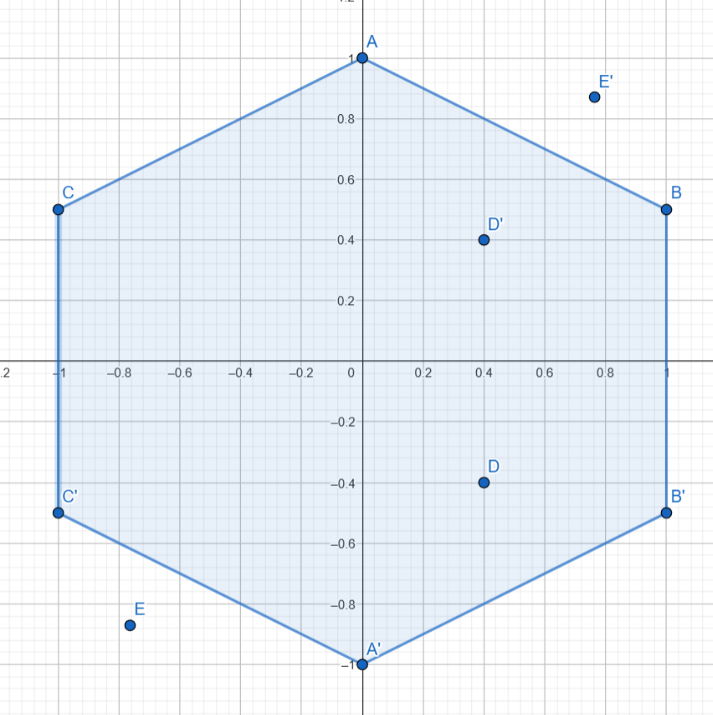
\includegraphics[width=.65\linewidth]{inside_hexagon.png}
    \caption{Schéma montrant l'effet des valeurs absolues dans la vérification de la position du clic de la souris à l'intérieur d'un hexagone. Les points D et E deviennent respectivement les points D' et E' lorsque la valeur absolue est appliquée. Il suffit seulement de vérifier que le point se trouve dans le quadrilatère formé par le point A, B, l'origine et l'intersection entre l'axe des abscisses et la perpendiculaire de B.}
    \label{fig:inside_hexagon}
\end{figure}

\bigskip
\item \textbf{Tests}

La disposition et le format de l’affichage du plateau ne sont pas testés. En revanche, un test vérifie l’initialisation du widget en s’assurant qu'elle appelle les méthodes de mise à jour de l’échelle et de dessin du plateau et qu’elle se passe sans erreur.
La méthode qui vérifie si un clic de la souris se trouve dans un hexagone depuis son carré est testée en simulant deux clics à chaque sommet et milieu de segment, un juste à l’extérieur et un juste à l’intérieur.
La gestion du clic est ensuite testée en simulant des clics en dehors du plateau et sur toutes les cases valides du plateau.
\end{enumerate}

\section{Menus de l'interface graphique} \label{annexe-gui}

\subsection{Menu principal}

Il s’agit de la première fenêtre qui s’ouvre au lancement du programme. Elle permet à l’utilisateur de charger une partie (F46), d’afficher la fenêtre d’aide (F46) ou la fenêtre ‘à propos’ (F48) et de quitter le programme (F46).  Le mode contest est également accessible depuis cette fenêtre. Pour démarrer une nouvelle partie, l’utilisateur doit accéder au menu New Game depuis le menu principal. Il pourra alors modifier la configuration du jeu avant de commencer. L’utilisateur peut également changer la langue du programme grâce au menu déroulant situé en bas à droite de cette fenêtre.
À chaque fois que cette fenêtre est affichée, on réinitialise l’état de GameState pour que le mode Contest puisse fonctionner correctement (le mode Contest vérifie qu’une partie est finie avant de suggérer un coup à jouer).

\begin{figure}[H]
    \centering
    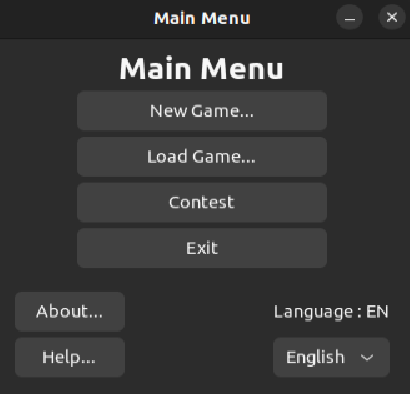
\includegraphics[width=.65\linewidth]{main_menu.png}
    \caption{Capture d'écran du menu principal de notre interface graphique.}
    \label{fig:menu-princ}
\end{figure}

\bigskip
Les tests du menu principal s’assurent qu’un clic sur les boutons affiche les fenêtres concernées et masque le menu principal. Il existe également un test permettant de vérifier si un changement de langue via l’interface utilisateur s’applique immédiatement, sans rafraîchir la fenêtre.

\bigskip
Le test des fenêtres About et Help consiste en deux classes TestAboutMenu et TestHelpMenu situées dans le fichier tests/test\_menus\_gui.py. Ces deux fenêtres étant assez proches par conception, leurs tests le sont également. Ces tests vérifient le titre de la fenêtre, la présence du bouton retour et si un clic sur ce bouton masque bien la fenêtre et affiche la fenêtre précédente.

\subsection{Menu ‘New Game’}
Cette fenêtre s’affiche entre le menu principal et la fenêtre de jeu. C’est ici que l’utilisateur peut régler chaque élément présent dans la section « Game » de la configuration. Dans la partie supérieure de la fenêtre, le joueur peut régler la taille du plateau, le mode blitz et le mode swap. La partie inférieure regroupe les réglages de l’intelligence artificielle. L’utilisateur a le choix entre un réglage simplifié où il peut choisir la difficulté de l’IA et un réglage avancé où il peut modifier tous les réglages de l’IA présents dans la section IA de la configuration (heuristique, profondeur de recherche…). Les onglets ‘Simple’ et ‘Avancé’ sont synchronisés pour une meilleure expérience utilisateur :
\begin{itemize}
    \item Quand l’utilisateur choisit une difficulté dans l’onglet ‘Simple’, les réglages correspondants sont automatiquement appliqués dans l’onglet ‘Avancé’.
    \item Quand l’utilisateur modifie les réglages de l’IA dans l’onglet ‘Avancé’, si la difficulté sélectionnée dans l’onglet ‘Simple’ est ‘None’, elle changera en ‘Custom’.
\end{itemize}

\begin{figure}[H]
    \centering
    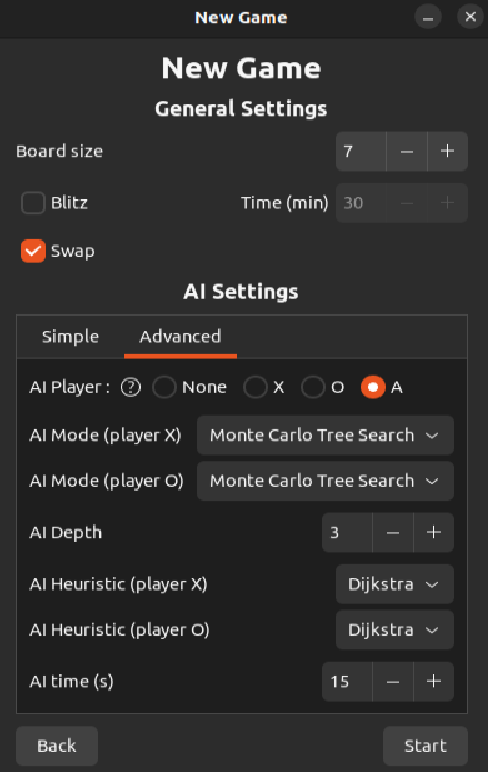
\includegraphics[width=.45\linewidth]{menu_new_game.png}
    \caption{Capture d'écran du menu ‘New Game’ de notre interface graphique.}
    \label{fig:menu-new}
\end{figure}

\bigskip
Au lancement d’une partie, une nouvelle instance de GameState est créée pour synchroniser les changements de configuration, notamment la taille du plateau qui est déterminée uniquement lors de son initialisation dans GameState.

\bigskip
Les tests de cette fenêtre s’assurent notamment qu’il n’est pas possible de lancer une partie avec des paramètres invalides et que les onglets « Simple » et « Avancé » de la section IA communiquent bien (si l’utilisateur choisit une difficulté pour l’IA, le joueur X doit être désigné comme joueur artificiel dans l’onglet ‘Avancé’ etc).

\subsection{Fenêtre de jeu}

La fenêtre de jeu est constituée d'une grille (Gtk.Grid) qui regroupe différents widgets :
\begin{itemize}
    \item Le plateau au centre (BoardWidget).
    \item Des textes pour l'affichage du joueur courant, des historiques et des timers (Gtk.label) en haut et sur le côtés de la fenêtre.
    \item Quatre boutons en bas de la fenêtre pour undo, redo, hint et pause.
\end{itemize}
La fonction hint dépend de l'IA couramment utilisée, qui peut donc prendre un certain temps avant de calculer le meilleur coup à jouer (cf. \ref{crit-connec}). Aussi, jouer un coup via une IA se fait par la création d'un thread qui va désactiver l’interaction avec la fenêtre le temps que l'IA joue. Ainsi, si les deux joueurs sont des IA, l’utilisateur ne pourra pas interagir avec la fenêtre tant que la partie ne sera pas achevée (il pourra toujours cliquer sur la croix pour fermer le programme).

\begin{figure}[H]
    \centering
    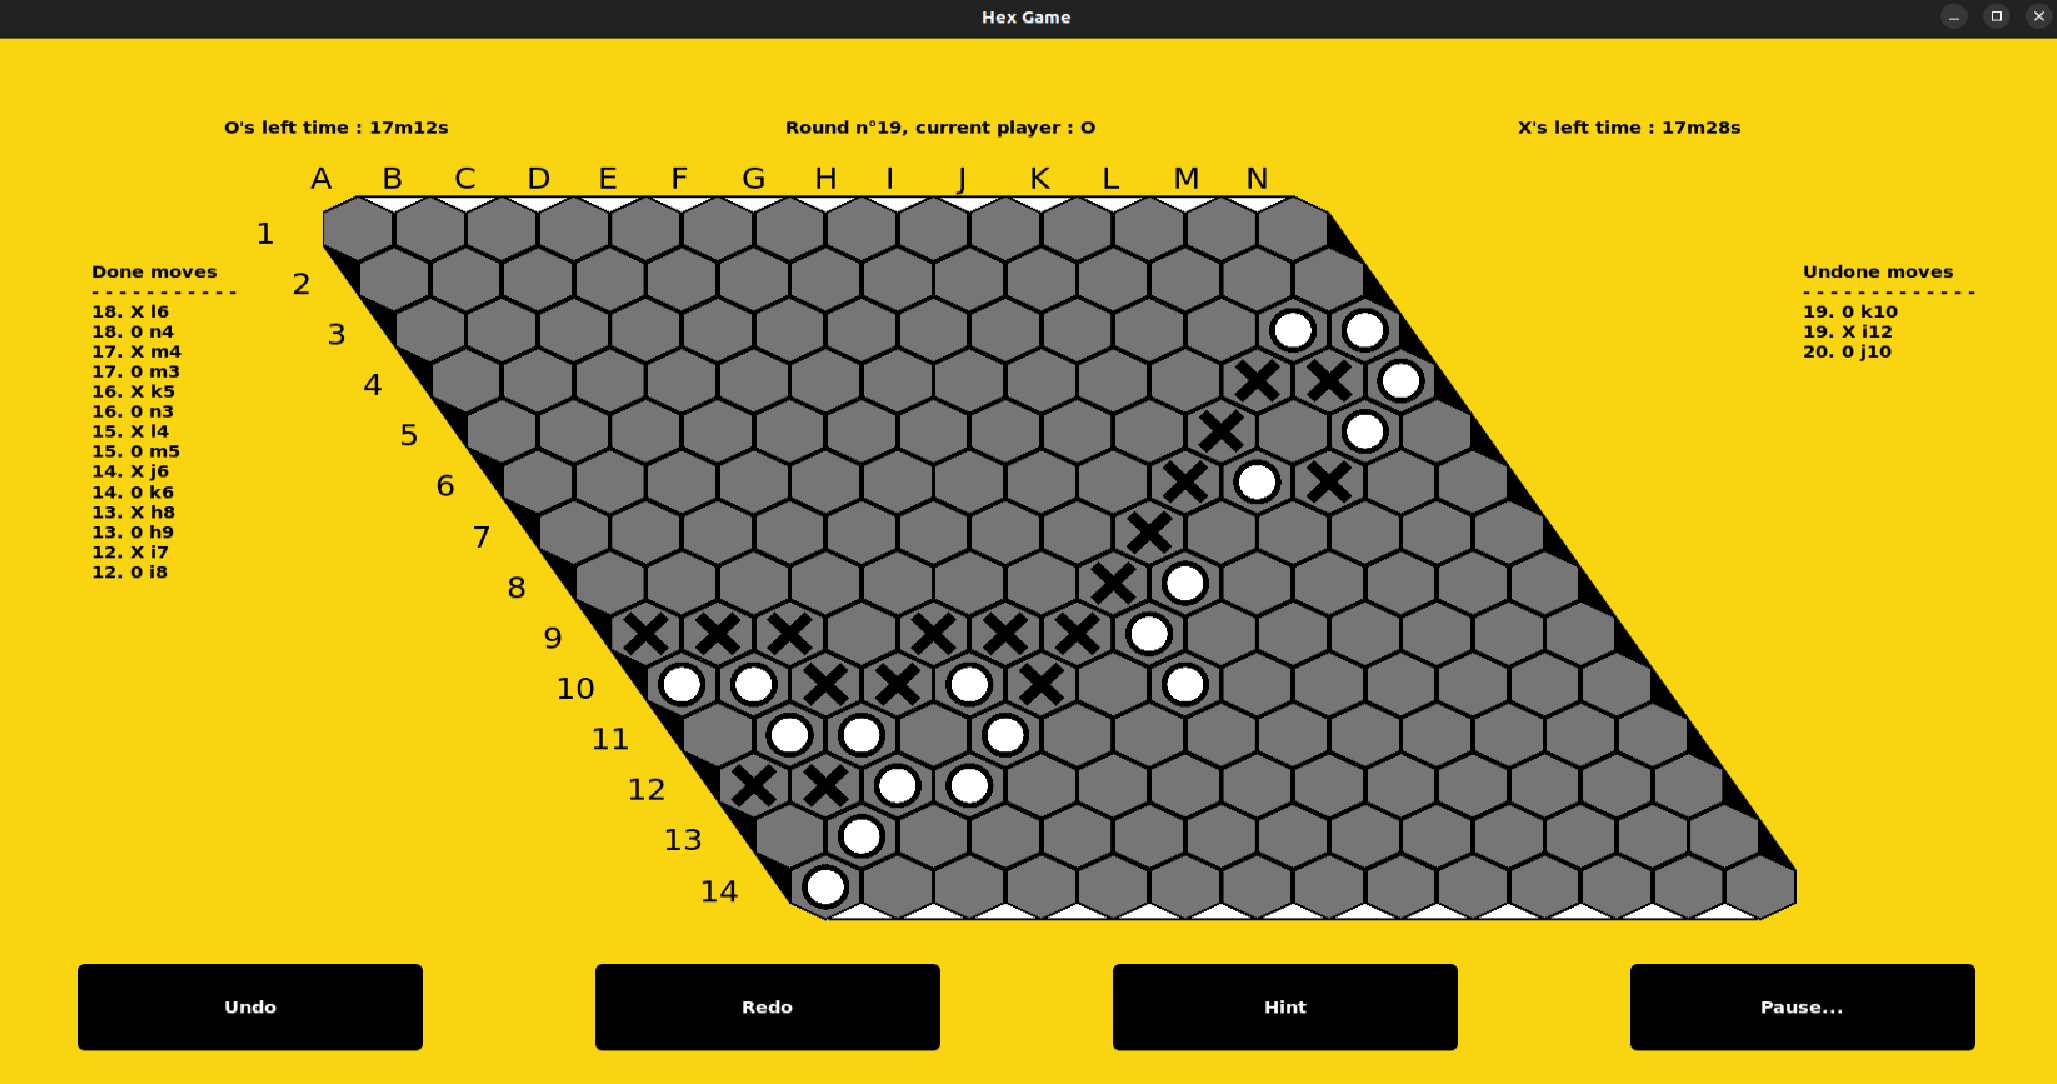
\includegraphics[width=1\linewidth]{game_gui.png}
    \caption{Capture d'écran de la fenêtre de jeu de notre interface graphique.}
    \label{fig:game_gui}
\end{figure}

\subsection{Menu Pause}

Ce menu est accessible uniquement lorsqu’une partie est en cours via le bouton situé en bas à droite de la fenêtre de jeu. Il met en pause le chronomètre du mode blitz si ce mode est activé et empêche l’utilisateur d'interagir avec le plateau de jeu. On y retrouve un bouton permettant de sauvegarder la partie en cours (F46) ainsi que d’autres fonctions de base comme la possibilité de redémarrer la partie en cours, d’abandonner ou encore de retourner au menu principal.

\begin{figure}[H]
    \centering
    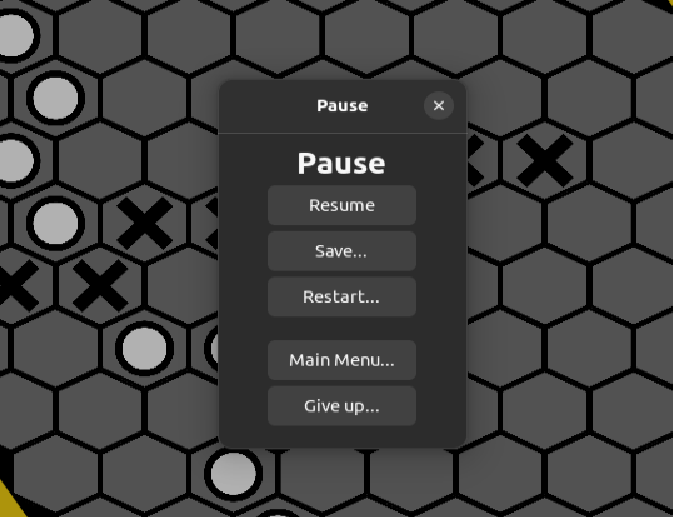
\includegraphics[width=.65\linewidth]{menu_pause.png}
    \caption{Capture d'écran du menu pause de la fenêtre de jeu de notre interface graphique.}
    \label{fig:menu-pause}
\end{figure}

\end{document}